\section{Introduction To Distributed Systems}
%%%%%%%%%%%%%%%%%%%%%%%%%%%%%%%%%%%%%%%%%%%%%%%%%%%%%%%
\subsection{Course Intro}
\begin{frame}
\frametitle{Chapter Objectives}

\begin{itemize} [<+->]
	\item Capturing the state of the art in building high performance distributed computing using Hadoop, Spark, and Kafka.
	\item Providing the relevant theoretical and practical background and its best practices.
	\item Demonastrating the main concepts and components for distributed systems. 
	\item Advancing the understanding of building scalable software systems for large scale data processing and its best practices. 
\end{itemize}

\end{frame}

%%%%%%%%%%%%%%%%%%%%%%%%%%%%%%%%%%%%%%%%%%%%%%%%%%%%%%

\begin{frame}
	\frametitle{Target Audience}
	
	\begin{itemize} [<+->]
		\item Software Engineers and Application Developers.
		\item Data Analysts and DWH/Data Engineers.
		\item Researchers.
	\end{itemize}
	
\end{frame}
%%%%%%%%%%%%%%%%%%%%%%%%%%%%%%%%%%%%%%%%%%%%%%%%%%%%%%


\subsection{Design Simple Distributed System (Case Study Example 1)}
\begin{frame}
	\frametitle{Case Study Example 1}
	\begin{itemize}  [<+->]
		\item Assume we have a file contains \textbf{\underline{1TB}} of text lines, and we need to convert the text to be the upper case, for example (The -> THE).
		\item We need to design the program without using any ready distributed system framework.
		\item You can use any number (n) of machines. Assume n specs are 8 GB of memory, hard desk 128 GB, and 2 cores of CPU.

	\end{itemize}
\end{frame}

%%%%%%%%%%%%%%%%%%%%%%%%%%%%%%%%%%%%%%%%%%%%%%%%%%%%%%
\begin{frame}[plain,c]
	\frametitle{Case Study Example 1}
		\begin{figure}
		\begin{center}




\tikzset{every picture/.style={line width=0.75pt}} %set default line width to 0.75pt        

\begin{tikzpicture}[x=0.75pt,y=0.75pt,yscale=-1,xscale=1]
	%uncomment if require: \path (0,212); %set diagram left start at 0, and has height of 212
	
	%Shape: Rectangle [id:dp3834116102870988] 
	\draw  [color={rgb, 255:red, 74; green, 144; blue, 226 }  ,draw opacity=1 ][line width=1]  (14,95) -- (105,95) -- (105,130) -- (14,130) -- cycle ;
	
	%Straight Lines [id:da7265782866155249] 
	\draw [color={rgb, 255:red, 155; green, 155; blue, 155 }  ,draw opacity=1 ][line width=0.75]    (109,113.5) -- (178,113.5) ;
	\draw [shift={(180 ,113.5)}, rotate = 180] [color={rgb, 255:red, 155; green, 155; blue, 155 }  ,draw opacity=1 ][line width=0.75]    (10.93,-3.29) .. controls (6.95,-1.4) and (3.31,-0.3) .. (0,0) .. controls (3.31,0.3) and (6.95,1.4) .. (10.93,3.29)   ;
	%%%PC start 
	%Shape: Frame [id:dp3239595123755211] 
	\draw  [color=offwhite  ,draw opacity=1 ][line width=0.75]  (188,86) -- (252,86) -- (252,126) -- (188,126) -- cycle(246,92) -- (194,92) -- (194,120) -- (246,120) -- cycle ;
	
	%Shape: Trapezoid [id:dp6832413050712917] 
	\draw  [color=offwhite  ,draw opacity=1 ][line width=0.75]  (178,156) -- (187,126) -- (253,126) -- (262,156) -- cycle ;
	
	%Shape: Trapezoid [id:dp7279166981904915] 
	\draw  [line width=0.75]  (182,152) -- (189.5,127) -- (250.5,127) -- (258,152) -- cycle ;
	%%%PC end 

	%Output
	%Shape: Rectangle [id:dp6681325814864821] 
	\draw  [color={rgb, 255:red, 70; green, 155; blue, 36 } ,draw opacity=1][line width=1]  (334,95) -- (425,95) -- (425,129) -- (334,129)  -- cycle ;


	%Straight Lines [id:da3966973170014948] 
	\draw [color={rgb, 255:red, 155; green, 155; blue, 155 }  ,draw opacity=1 ][line width=0.75]    (257,113.5) -- (323,113.5) ;
	\draw [shift={(326,113.5)}, rotate = 180] [color={rgb, 255:red, 155; green, 155; blue, 155 }  ,draw opacity=1 ][line width=0.75]    (10.93,-3.29) .. controls (6.95,-1.4) and (3.31,-0.3) .. (0,0) .. controls (3.31,0.3) and (6.95,1.4) .. (10.93,3.29)   ;
	
	% Text Node
	\draw (45,160) node [anchor=north west][inner sep=0.75pt]  [font=\footnotesize,color={rgb, 255:red, 74; green, 144; blue, 226 }  ,opacity=1 ] [align=center] {Input};
	% Text Node
	\draw (33,107) node [anchor=north west][inner sep=0.75pt]  [font=\scriptsize,color={rgb, 255:red, 74; green, 144; blue, 226 }  ,opacity=1 ] [align=center] {Hello world};
	% Text Node
	\draw (210,163) node [anchor=north west][inner sep=0.75pt]  [font=\footnotesize,color=offwhite] [align=left] {PC};
	% Text Node
	\draw (340,107) node [anchor=north west][inner sep=0.75pt]  [font=\scriptsize,color={rgb, 255:red, 70; green, 155; blue, 36}  ,opacity=1 ] [align=center] {HELLO WORLD};
	% Text Node
	\draw (360,160) node [anchor=north west][inner sep=0.75pt]  [font=\footnotesize,color={rgb, 255:red, 70; green, 155; blue, 36 }  ,opacity=1 ] [align=center] {Output};
	
	
\end{tikzpicture}
\end{center}

		\caption{Simple design for small file(s) processing } \label{fig:DS1}
		\end{figure}
\end{frame}
%%%%%%%%%%%%%%%%%%%%%%%%%%%%%%%%%%%%%%%%%%%%%%%%%%%%%%
\begin{frame}[plain,c]
	\frametitle{Case Study Example 1}
	\begin{figure}
		\centering
		


\tikzset{every picture/.style={line width=0.75pt}} %set default line width to 0.75pt        

\begin{tikzpicture}[x=0.75pt,y=0.75pt,yscale=-1,xscale=1]
	%uncomment if require: \path (0,415); %set diagram left start at 0, and has height of 415
	
	%Shape: Rectangle [id:dp8655887794683795] 
	\draw  [color={rgb, 255:red, 65; green, 117; blue, 5 }  ,draw opacity=1 ] (18,111) -- (252.58,111) -- (252.58,202.25) -- (18,202.25) -- cycle ;
	%Shape: Rectangle [id:dp8907085252035312] 
	\draw  [color={rgb, 255:red, 65; green, 117; blue, 5 }  ,draw opacity=1 ] (302.58,111) -- (362.58,111) -- (362.58,201.75) -- (302.58,201.75) -- cycle ;
	%Shape: Rectangle [id:dp531973268669913] 
	\draw  [color={rgb, 255:red, 80; green, 227; blue, 194 }  ,draw opacity=1 ] (50,121) -- (90,121) -- (90,141) -- (50,141) -- cycle ;
	%Shape: Rectangle [id:dp32192612836678103] 
	\draw  [color={rgb, 255:red, 80; green, 227; blue, 194 }  ,draw opacity=1 ] (110,121) -- (150,121) -- (150,141) -- (110,141) -- cycle ;
	%Shape: Rectangle [id:dp972266177760866] 
	\draw  [color={rgb, 255:red, 80; green, 227; blue, 194 }  ,draw opacity=1 ] (170,121) -- (210,121) -- (210,141) -- (170,141) -- cycle ;
	%Rounded Rect [id:dp763489432971651] 
	\draw  [color={rgb, 255:red, 208; green, 2; blue, 27 }  ,draw opacity=1 ] 
	 (50,175) -- (210,175) -- (210,195) -- (50,195) -- cycle ;-- cycle ;
	%Shape: Rectangle [id:dp46420165615263753] 
	\draw  [color={rgb, 255:red, 65; green, 117; blue, 5 }  ,draw opacity=1 ] (480.58,111) -- (542.58,111) -- (542.58,200.75) -- (480.58,200.75) -- cycle ;
	%Shape: Rectangle [id:dp27479252331465176] 
	\draw  [color={rgb, 255:red, 65; green, 117; blue, 5 }  ,draw opacity=1 ] (393.58,177) -- (455.58,177) -- (455.58,266.75) -- (393.58,266.75) -- cycle ;
	%Straight Lines [id:da369260676335904] 
	\draw [line width=2.25]    (279.58,73.25) -- (280.58,207.25) ;
	%Shape: Rectangle [id:dp7935185593682178] 
	\draw  [color={rgb, 255:red, 80; green, 227; blue, 194 }  ,draw opacity=1 ] (310,121) -- (350,121) -- (350,140) -- (310,140) -- cycle ;
	%Shape: Rectangle [id:dp34622696632931327]   % memory box 2
	\draw  [color={rgb, 255:red, 208; green, 2; blue, 27 }  ,draw opacity=1 ] (310,175) -- (350,175) -- (350,195) -- (310,195) -- cycle ;
	%Shape: Rectangle [id:dp00038374666294560544] 
	\draw  [color={rgb, 255:red, 80; green, 227; blue, 194 }  ,draw opacity=1 ] (405,190) -- (445,190) -- (445,210) -- (405,210) -- cycle ;
	%Shape: Rectangle [id:dp3209647982053657] 
	\draw  [color={rgb, 255:red, 80; green, 227; blue, 194 }  ,draw opacity=1 ] (490,121) -- (530,121) -- (530,141) -- (490,141) -- cycle ;
	%Shape: Rectangle [id:dp8025652037528683]  %memory box 4
	\draw  [color={rgb, 255:red, 208; green, 2; blue, 27 }  ,draw opacity=1 ] (405.58,236.25) -- (443.58,236.25) -- (443.58,257.25) -- (405.58,257.25) -- cycle ;
	%Shape: Rectangle [id:dp2266373468363876]  % memory box 3
	\draw  [color={rgb, 255:red, 208; green, 2; blue, 27 }  ,draw opacity=1 ] (490,175) -- (530,175) -- (530,195) -- (490,195) -- cycle ;
	%Straight Lines [id:da5029820921379233] 
	\draw    [color=offyellow, <->]  (331.58,141) -- (331.58,175) ;

	%Straight Lines [id:da9994794173682501] 
	\draw  [color=offyellow, <->]  (511.58,141) -- (511.58,175) ;
	%Straight Lines [id:da9705771813095805] 
	\draw  [color=offyellow, <->]   (186.58,141) -- (186.58,175) ;
	%Straight Lines [id:da5879748150918536] 
	\draw  [color=offyellow, <->]   (129.58,141) -- (129.58,175) ;
	%Straight Lines [id:da6653546271183027] 
	\draw [color=offyellow, <->]    (70,141) -- (70,175) ;


	%Straight Lines [id:da7730658410797611] 
	\draw   [color=offyellow, <->]  (424.58,210) -- (424.58,236.25) ;

	%Straight Lines [id:da9386491963364736] 
	\draw   [color=offyellow, <->]  (366.58,162.75) -- (389.43,195.12) ;
	%Straight Lines [id:da5731244822727878] 
	\draw   [color=offyellow, <->]  (477.58,165.75) -- (457.59,200.02) ;
	%Straight Lines [id:da06900608847320588] 
	\draw  [color=offyellow, <->]   (479.58,135.75) -- (366.58,134.77) ;
	
	% Text Node
	\draw (90,87) node [anchor=north west][inner sep=0.75pt]   [align=left] {Parallel};
	% Text Node
	\draw (335,87) node [anchor=north west][inner sep=0.75pt]   [align=left] {Distributed Processing};
	% Text Node
	\draw (114.42,180) node [anchor=north west][inner sep=0.75pt]  [font=\tiny,xslant=-0.07] [align=left] {\textbf{Memory}};
	% Text Node
	\draw (313.5,180) node [anchor=north west][inner sep=0.75pt]  [font=\tiny,xslant=-0.07] [align=left] {\textbf{Memory}};
	% Text Node
	\draw (53.5,126) node [anchor=north west][inner sep=0.75pt]   [align=left] {{\tiny \textbf{Process}}};
	% Text Node
	\draw (113.5,126) node [anchor=north west][inner sep=0.75pt]   [align=left] {{\tiny \textbf{Process}}};
	% Text Node
	\draw (173.5,126) node [anchor=north west][inner sep=0.75pt]   [align=left] {{\tiny \textbf{Process}}};
	% Text Node
	\draw (313.5,126) node [anchor=north west][inner sep=0.75pt]   [align=left] {{\tiny \textbf{Process}}};
	% Text Node
	\draw (408.5,195) node [anchor=north west][inner sep=0.75pt]   [align=left] {{\tiny \textbf{Process}}};
	% Text Node
	\draw (493.5,126) node [anchor=north west][inner sep=0.75pt]   [align=left] {{\tiny \textbf{Process}}};
	% Text Node
	\draw (408,242) node [anchor=north west][inner sep=0.75pt]  [font=\tiny,xslant=-0.07] [align=left] {\textbf{Memory}};
	% Text Node
	\draw (493.5,180) node [anchor=north west][inner sep=0.75pt]  [font=\tiny,xslant=-0.07] [align=left] {\textbf{Memory}};
	
	
\end{tikzpicture}

		\label{fig:DS2}
		\caption{Parallel processing vs Distributed processing } 
	\end{figure}
\end{frame}
%%%%%%%%%%%%%%%%%%%%%%%%%%%%%%%%%%%%%%%%%%%%%%%%%%%%%%
\begin{frame}[plain,c]
	\frametitle{Case Study Example 1}
		\begin{figure}
		\centering
			


\tikzset{every picture/.style={line width=0.75pt}} %set default line width to 0.75pt        

\begin{tikzpicture}[x=0.75pt,y=0.75pt,yscale=-1,xscale=1]
	%uncomment if require: \path (0,300); %set diagram left start at 0, and has height of 300

	%input
	%Shape: Rectangle [id:dp6258708726014198] 
	\draw  [color={rgb, 255:red, 74; green, 144; blue, 226 }  ,draw opacity=1 ][line width=1.5]  (11,150) -- (100,150) -- (100,189.67) -- (11,189.67) -- cycle ;

	%Shape: Frame [id:dp45199805556426453] 
	\draw [color=offwhite] [line width=0.75]  (353,131) -- (417,131) -- (417,171) -- (353,171) -- cycle(411,137) -- (359,137) -- (359,165) -- (411,165) -- cycle ;
	%Shape: Trapezoid [id:dp6365442083669953] 
	\draw  [color=offwhite]  [line width=0.75]  (343,201) -- (352,171) -- (418,171) -- (427,201) -- cycle ;
	%Shape: Trapezoid [id:dp7035229008077436] 
	\draw   [color=offwhite] [line width=0.75]  (347,197) -- (354.5,172) -- (415.5,172) -- (423,197) -- cycle ;
	
	%output
	%Shape: Rectangle [id:dp4075005896181748] 
	\draw  [color={rgb, 255:red, 70; green, 155; blue, 36 }  ,draw opacity=1 ][line width=1.5]  (470.75,150) -- (560,150) -- (560,189) -- (470.75,189) -- cycle ;
	
	%Straight Lines [id:da6139983456591827]  Node1->Output
	\draw [color={rgb, 255:red, 155; green, 155; blue, 155 }  ,draw opacity=1 ][line width=0.75]    (418,169) -- (464,169) ;
	\draw [shift={(465,169)}, rotate = 539.64] [color={rgb, 255:red, 155; green, 155; blue, 155 }  ,draw opacity=1 ][line width=0.75]    (10.93,-3.29) .. controls (6.95,-1.4) and (3.31,-0.3) .. (0,0) .. controls (3.31,0.3) and (6.95,1.4) .. (10.93,3.29)   ;
	
	
	%Straight Lines [id:da7123818425757267] 
	\draw [color={rgb, 255:red, 128; green, 128; blue, 128 }  ,draw opacity=1 ]   (101,169) -- (128.88,169) ;
	\draw [shift={(130.88,169)}, rotate = 539.6800000000001] [color={rgb, 255:red, 128; green, 128; blue, 128 }  ,draw opacity=1 ][line width=0.75]    (10.93,-3.29) .. controls (6.95,-1.4) and (3.31,-0.3) .. (0,0) .. controls (3.31,0.3) and (6.95,1.4) .. (10.93,3.29)   ;
	
	%Shape: Rectangle [id:dp9860882909394741] 
	\draw  [color=offred  ,draw opacity=1 ][line width=0.75]  (230.75,119.63) -- (300.75,119.63) -- (300.75,149.63) -- (230.75,149.63) -- cycle ;
	%Shape: Rectangle [id:dp6809508870305205] 
	\draw  [color=offred  ,draw opacity=1 ][line width=0.75]  (229.75,189.63) -- (300.75,189.63) -- (300.75,219.63) -- (229.75,219.63) -- cycle ;
	%Curve Lines [id:da19696995243819926] 
	\draw [color={rgb, 255:red, 128; green, 128; blue, 128 }  ,draw opacity=1 ]   (169.75,190.63) .. controls (177.42,212.05) and (183.62,223.4) .. (228.38,219.75) ;
	\draw [shift={(229.75,219.63)}, rotate = 535.03] [color={rgb, 255:red, 128; green, 128; blue, 128 }  ,draw opacity=1 ][line width=0.75]    (10.93,-3.29) .. controls (6.95,-1.4) and (3.31,-0.3) .. (0,0) .. controls (3.31,0.3) and (6.95,1.4) .. (10.93,3.29)   ;
	%Curve Lines [id:da14087388365596432] 
	\draw [color={rgb, 255:red, 128; green, 128; blue, 128 }  ,draw opacity=1 ]   (169.75,149.63) .. controls (169.75,139.73) and (185.43,114.15) .. (229.41,119.46) ;
	\draw [shift={(230.75,119.63)}, rotate = 187.59] [color={rgb, 255:red, 128; green, 128; blue, 128 }  ,draw opacity=1 ][line width=0.75]    (10.93,-3.29) .. controls (6.95,-1.4) and (3.31,-0.3) .. (0,0) .. controls (3.31,0.3) and (6.95,1.4) .. (10.93,3.29)   ;
	%Curve Lines [id:da6655261202271237] 
	\draw [color={rgb, 255:red, 128; green, 128; blue, 128 }  ,draw opacity=1 ]   (300.75,119.63) .. controls (311.59,149.18) and (317.57,170) .. (351.43,170.97) ;
	\draw [shift={(353,171)}, rotate = 180.6] [color={rgb, 255:red, 128; green, 128; blue, 128 }  ,draw opacity=1 ][line width=0.75]    (10.93,-3.29) .. controls (6.95,-1.4) and (3.31,-0.3) .. (0,0) .. controls (3.31,0.3) and (6.95,1.4) .. (10.93,3.29)   ;
	%Curve Lines [id:da188937268210565] 
	\draw [color={rgb, 255:red, 128; green, 128; blue, 128 }  ,draw opacity=1 ]   (300.75,219.63) .. controls (310.55,191.21) and (318.43,171.44) .. (350.04,171) ;
	\draw [shift={(352,171)}, rotate = 180.63] [color={rgb, 255:red, 128; green, 128; blue, 128 }  ,draw opacity=1 ][line width=0.75]    (10.93,-3.29) .. controls (6.95,-1.4) and (3.31,-0.3) .. (0,0) .. controls (3.31,0.3) and (6.95,1.4) .. (10.93,3.29)   ;
	%Shape: Rectangle [id:dp795964462639149] 
	\draw  [color=offyellow ,draw opacity=1 ] (134,150) -- (205,150) -- (205,190) -- (134,190) -- cycle ;
	
	% Text Node
	\draw (38,208) node [anchor=north west][inner sep=0.75pt]  [font=\footnotesize,color={rgb, 255:red, 74; green, 144; blue, 226 }  ,opacity=1 ] [align=left] {Input};
	% Text Node
	\draw (28,164) node [anchor=north west][inner sep=0.75pt]  [font=\scriptsize,color={rgb, 255:red, 74; green, 144; blue, 226 }  ,opacity=1 ] [align=left] {Hello world};
	% Text Node
	\draw (364,208) node [anchor=north west][inner sep=0.75pt]  [font=\footnotesize] [align=left] {Node 1};
	% Text Node
	\draw (477,164) node [anchor=north west][inner sep=0.75pt]  [font=\scriptsize,color={rgb, 255:red, 70; green, 155; blue, 36 }  ,opacity=1 ] [align=left] {HELLO WORLD};
	% Text Node
	\draw (496,208) node [anchor=north west][inner sep=0.75pt]  [font=\footnotesize,color={rgb, 255:red, 70; green, 155; blue, 36 }  ,opacity=1 ] [align=left] {Output};
	% Text Node
	\draw (148,164) node [anchor=north west][inner sep=0.75pt]  [font=\scriptsize,color=offyellow  ,opacity=1 ] [align=left] {File Split};
	% Text Node
	\draw (248,131) node [anchor=north west][inner sep=0.75pt]  [font=\scriptsize,color=offred  ,opacity=1 ] [align=left] {Split-1};
	% Text Node
	\draw (248,200) node [anchor=north west][inner sep=0.75pt]  [font=\scriptsize,color=offred  ,opacity=1 ] [align=left] {Split-2};
	
	
	
\end{tikzpicture}

			\caption{Adding File Split function to split big files into equal chunks } \label{fig:DS3}
		\end{figure}

\end{frame}
%%%%%%%%%%%%%%%%%%%%%%%%%%%%%%%%%%%%%%%%%%%%%%%%%%%%%%
\begin{frame}[plain,c]
	\frametitle{Case Study Example 1}
		\begin{figure}
		\centering
			


\tikzset{every picture/.style={line width=0.75pt}} %set default line width to 0.75pt        

\begin{tikzpicture}[scale=0.95,x=0.75pt,y=0.75pt,yscale=-1,xscale=1]
	%uncomment if require: \path (0,300); %set diagram left start at 0, and has height of 300
	
	%Shape: Rectangle [id:dp6258708726014198] 
	\draw  [color={rgb, 255:red, 74; green, 144; blue, 226 }  ,draw opacity=1 ][line width=1.5]  (60,151) -- (100,151) -- (100,189.67) -- (60,189.67) -- cycle ;

    %Node1
	%Shape: Frame [id:dp45199805556426453] 
	\draw  [line width=0.75,color=offwhite]  (445,57) -- (509,57) -- (509,97) -- (445,97) -- cycle(503,63) -- (451,63) -- (451,91) -- (503,91) -- cycle ;
	%Shape: Trapezoid [id:dp6365442083669953] 
	\draw  [line width=0.75,color=offwhite]  (435,127) -- (444,97) -- (510,97) -- (519,127) -- cycle ;
	%Shape: Trapezoid [id:dp7035229008077436] 
	\draw  [line width=0.75,color=offwhite]  (439,123) -- (446.5,98) -- (507.5,98) -- (515,123) -- cycle ;
	
    %Shape: Rectangle [id:dp4075005896181748] 
	\draw  [color={rgb, 255:red, 70; green, 155; blue, 36 }  ,draw opacity=1 ][line width=1.5]  (560.75,151) -- (610,151) -- (610,189) -- (560.75,189) -- cycle ;
	
    %output
    %Straight Lines [id:da7123818425757267] 
	\draw [color={rgb, 255:red, 128; green, 128; blue, 128 }  ,draw opacity=1 ]   (101,170) -- (128.88,169.84) ;
	\draw [shift={(130.88,169.83)}, rotate = 539.6800000000001] [color={rgb, 255:red, 128; green, 128; blue, 128 }  ,draw opacity=1 ][line width=0.75]    (10.93,-3.29) .. controls (6.95,-1.4) and (3.31,-0.3) .. (0,0) .. controls (3.31,0.3) and (6.95,1.4) .. (10.93,3.29)   ;
	
    %Shape: Rectangle [id:dp9860882909394741] 
	\draw  [color=offred  ,draw opacity=1 ][line width=0.75]  (230.75,119.63) -- (300.75,119.63) -- (300.75,149.63) -- (230.75,149.63) -- cycle ;
	%Shape: Rectangle [id:dp6809508870305205] 
	\draw  [color=offred  ,draw opacity=1 ][line width=0.75]  (229.75,189.63) -- (300.75,189.63) -- (300.75,219.63) -- (229.75,219.63) -- cycle ;
	
    %Curve Lines [id:da19696995243819926] 
	\draw [color={rgb, 255:red, 128; green, 128; blue, 128 }  ,draw opacity=1 ]   (169.75,190.63) .. controls (177.42,212.05) and (183.62,223.4) .. (228.38,219.75) ;
	\draw [shift={(229.75,219.63)}, rotate = 535.03] [color={rgb, 255:red, 128; green, 128; blue, 128 }  ,draw opacity=1 ][line width=0.75]    (10.93,-3.29) .. controls (6.95,-1.4) and (3.31,-0.3) .. (0,0) .. controls (3.31,0.3) and (6.95,1.4) .. (10.93,3.29)   ;
	%Curve Lines [id:da14087388365596432] 
	\draw [color={rgb, 255:red, 128; green, 128; blue, 128 }  ,draw opacity=1 ]   (169.75,149.63) .. controls (169.75,139.73) and (185.43,114.15) .. (229.41,119.46) ;
	\draw [shift={(230.75,119.63)}, rotate = 187.59] [color={rgb, 255:red, 128; green, 128; blue, 128 }  ,draw opacity=1 ][line width=0.75]    (10.93,-3.29) .. controls (6.95,-1.4) and (3.31,-0.3) .. (0,0) .. controls (3.31,0.3) and (6.95,1.4) .. (10.93,3.29)   ;
	%Curve Lines [id:da6655261202271237] 
	\draw [color={rgb, 255:red, 128; green, 128; blue, 128 }  ,draw opacity=1 ]   (300.75,119.63) .. controls (311.59,149.18) and (302.77,169.68) .. (336.19,170.64) ;
	\draw [shift={(337.75,170.67)}, rotate = 180.6] [color={rgb, 255:red, 128; green, 128; blue, 128 }  ,draw opacity=1 ][line width=0.75]    (10.93,-3.29) .. controls (6.95,-1.4) and (3.31,-0.3) .. (0,0) .. controls (3.31,0.3) and (6.95,1.4) .. (10.93,3.29)   ;
	%Curve Lines [id:da188937268210565] 
	\draw [color={rgb, 255:red, 128; green, 128; blue, 128 }  ,draw opacity=1 ]   (300.75,219.63) .. controls (310.55,191.21) and (304.74,171.12) .. (335.8,170.67) ;
	\draw [shift={(337.75,170.67)}, rotate = 180.63] [color={rgb, 255:red, 128; green, 128; blue, 128 }  ,draw opacity=1 ][line width=0.75]    (10.93,-3.29) .. controls (6.95,-1.4) and (3.31,-0.3) .. (0,0) .. controls (3.31,0.3) and (6.95,1.4) .. (10.93,3.29)   ;
	
    %Shape: Rectangle [id:dp795964462639149] 
	\draw  [color=offyellow  ,draw opacity=1 ] (131,151) -- (201,151) -- (201,190) -- (131,190) -- cycle ;

	%Shape: Frame [id:dp7417485861438164] 
	\draw  [line width=0.75,color=offwhite]  (443,212) -- (507,212) -- (507,252) -- (443,252) -- cycle(501,218) -- (449,218) -- (449,246) -- (501,246) -- cycle ;
	%Shape: Trapezoid [id:dp7528630303015812] 
	\draw  [line width=0.75,color=offwhite]  (433,282) -- (442,252) -- (508,252) -- (517,282) -- cycle ;
	%Shape: Trapezoid [id:dp8885841590443699] 
	\draw  [line width=0.75,color=offwhite]  (437,278) -- (444.5,253) -- (505.5,253) -- (513,278) -- cycle ;

    %????
	%Shape: Rectangle [id:dp6221340422393318] 
	\draw  [color=offpurple,line width=0.75] (340,151) -- (389.75,151) -- (389.75,189.67) -- (340,189.67) -- cycle ;

	%Curve Lines [id:da17799352827092774] 
	\draw [color={rgb, 255:red, 128; green, 128; blue, 128 }  ,draw opacity=1 ]   (390,170.17) .. controls (415.99,126.11) and (392.72,97.25) .. (442.47,97) ;
	\draw [shift={(444,97)}, rotate = 180.37] [color={rgb, 255:red, 128; green, 128; blue, 128 }  ,draw opacity=1 ][line width=0.75]    (10.93,-3.29) .. controls (6.95,-1.4) and (3.31,-0.3) .. (0,0) .. controls (3.31,0.3) and (6.95,1.4) .. (10.93,3.29)   ;
	
    %Curve Lines [id:da9685723605797839] 
	\draw [color={rgb, 255:red, 128; green, 128; blue, 128 }  ,draw opacity=1 ]   (390,170.17) .. controls (415.86,237.64) and (399.75,251.26) .. (440.12,251.98) ;
	\draw [shift={(442,252)}, rotate = 180.45] [color={rgb, 255:red, 128; green, 128; blue, 128 }  ,draw opacity=1 ][line width=0.75]    (10.93,-3.29) .. controls (6.95,-1.4) and (3.31,-0.3) .. (0,0) .. controls (3.31,0.3) and (6.95,1.4) .. (10.93,3.29)   ;
	
    %Curve Lines [id:da43813209116711305] 
	\draw [color={rgb, 255:red, 128; green, 128; blue, 128 }  ,draw opacity=1 ]   (510,97) .. controls (541.27,124.58) and (518.46,169.62) .. (557,172.88) ;
	\draw [shift={(558,173)}, rotate = 182.66] [color={rgb, 255:red, 128; green, 128; blue, 128 }  ,draw opacity=1 ][line width=0.75]    (10.93,-3.29) .. controls (6.95,-1.4) and (3.31,-0.3) .. (0,0) .. controls (3.31,0.3) and (6.95,1.4) .. (10.93,3.29)   ;
	
    %Curve Lines [id:da5479643719173531] 
	\draw [color={rgb, 255:red, 128; green, 128; blue, 128 }  ,draw opacity=1 ]   (508,252) .. controls (536.96,209.1) and (511.27,191.36) .. (557,173.54) ;
	\draw [shift={(558,173)}, rotate = 520.2] [color={rgb, 255:red, 128; green, 128; blue, 128 }  ,draw opacity=1 ][line width=0.75]    (10.93,-3.29) .. controls (6.95,-1.4) and (3.31,-0.3) .. (0,0) .. controls (3.31,0.3) and (6.95,1.4) .. (10.93,3.29)   ;
	

	% Text Node
	\draw (65,208) node [anchor=north west][inner sep=0.75pt]  [font=\footnotesize,color={rgb, 255:red, 74; green, 144; blue, 226 }  ,opacity=1 ]  {Input};
	% Text Node
	\draw (65,164) node [anchor=north west][inner sep=0.75pt]  [font=\scriptsize,color={rgb, 255:red, 74; green, 144; blue, 226 }  ,opacity=1 ]  {Hello};
	% Text Node
	\draw (454,131) node [anchor=north west][inner sep=0.75pt]  [font=\footnotesize,color=offwhite]  {Node 1};
	% Text Node
	\draw (564,167) node [anchor=north west][inner sep=0.75pt]  [font=\scriptsize,color={rgb, 255:red, 70; green, 155; blue, 36 }  ,opacity=1 ]  {HELLO};
	% Text Node
	\draw (564,208) node [anchor=north west][inner sep=0.75pt]  [font=\footnotesize,color={rgb, 255:red, 70; green, 155; blue, 36 }  ,opacity=1 ]  {Output};
	% Text Node
	\draw (141,164) node [anchor=north west][inner sep=0.75pt]  [font=\scriptsize,color=offyellow  ,opacity=1 ]  {File Split};
	% Text Node
	\draw (248,131) node [anchor=north west][inner sep=0.75pt]  [font=\scriptsize,color=offred  ,opacity=1 ]  {Split-1};
	% Text Node
	\draw (248,200) node [anchor=north west][inner sep=0.75pt]  [font=\scriptsize,color=offred  ,opacity=1 ]  {Split-2};
	% Text Node
	\draw (454,286) node [anchor=north west][inner sep=0.75pt]  [font=\footnotesize,color=offwhite]  {Node 2};
	% Text Node
	\draw (346,165) node [anchor=north west][inner sep=0.75pt]  [font=\scriptsize,color=offpurple]  {$S_x$ \% n };
    \draw (340,210) node [anchor=north west][inner sep=0.75pt]  [font=\scriptsize,color=offpurple]  {Mgmt Box};

    
	
\end{tikzpicture}

			\caption{Adding another node to distribute the processing across serveral nodes (n). } \label{fig:DS3}
		\end{figure}

\end{frame}
%%%%%%%%%%%%%%%%%%%%%%%%%%%%%%%%%%%%%%%%%%%%%%%%%%%%%%
\begin{frame}[plain,c]
	\frametitle{Case Study Example 1}
	\begin{figure}
		\centering
		


\tikzset{every picture/.style={line width=0.75pt}} %set default line width to 0.75pt        

\begin{tikzpicture}[scale=0.95,x=0.75pt,y=0.75pt,yscale=-1,xscale=1]
	%uncomment if require: \path (0,300); %set diagram left start at 0, and has height of 300
	
	%Shape: Rectangle [id:dp6258708726014198] 
	\draw  [color={rgb, 255:red, 74; green, 144; blue, 226 }  ,draw opacity=1 ][line width=1.5]  (60,151) -- (100,151) -- (100,189.67) -- (60,189.67) -- cycle ;

    %Node1
	%Shape: Frame [id:dp45199805556426453] 
	\draw  [line width=0.75,color=offwhite]  (445,57) -- (509,57) -- (509,97) -- (445,97) -- cycle(503,63) -- (451,63) -- (451,91) -- (503,91) -- cycle ;
	%Shape: Trapezoid [id:dp6365442083669953] 
	\draw  [line width=0.75,color=offwhite]  (435,127) -- (444,97) -- (510,97) -- (519,127) -- cycle ;
	%Shape: Trapezoid [id:dp7035229008077436] 
	\draw  [line width=0.75,color=offwhite]  (439,123) -- (446.5,98) -- (507.5,98) -- (515,123) -- cycle ;
	
    %Shape: Rectangle [id:dp4075005896181748] 
	\draw  [color={rgb, 255:red, 70; green, 155; blue, 36 }  ,draw opacity=1 ][line width=1.5]  (560.75,151) -- (610,151) -- (610,189) -- (560.75,189) -- cycle ;
	
    %output
    %Straight Lines [id:da7123818425757267] 
	\draw [color={rgb, 255:red, 128; green, 128; blue, 128 }  ,draw opacity=1 ]   (101,170) -- (128.88,169.84) ;
	\draw [shift={(130.88,169.83)}, rotate = 539.6800000000001] [color={rgb, 255:red, 128; green, 128; blue, 128 }  ,draw opacity=1 ][line width=0.75]    (10.93,-3.29) .. controls (6.95,-1.4) and (3.31,-0.3) .. (0,0) .. controls (3.31,0.3) and (6.95,1.4) .. (10.93,3.29)   ;
	
    %Shape: Rectangle [id:dp9860882909394741] 
	\draw  [color=offred  ,draw opacity=1 ][line width=0.75]  (230.75,119.63) -- (300.75,119.63) -- (300.75,149.63) -- (230.75,149.63) -- cycle ;
	%Shape: Rectangle [id:dp6809508870305205] 
	\draw  [color=offred  ,draw opacity=1 ][line width=0.75]  (229.75,189.63) -- (300.75,189.63) -- (300.75,219.63) -- (229.75,219.63) -- cycle ;
	
    %Curve Lines [id:da19696995243819926] 
	\draw [color={rgb, 255:red, 128; green, 128; blue, 128 }  ,draw opacity=1 ]   (169.75,190.63) .. controls (177.42,212.05) and (183.62,223.4) .. (228.38,219.75) ;
	\draw [shift={(229.75,219.63)}, rotate = 535.03] [color={rgb, 255:red, 128; green, 128; blue, 128 }  ,draw opacity=1 ][line width=0.75]    (10.93,-3.29) .. controls (6.95,-1.4) and (3.31,-0.3) .. (0,0) .. controls (3.31,0.3) and (6.95,1.4) .. (10.93,3.29)   ;
	%Curve Lines [id:da14087388365596432] 
	\draw [color={rgb, 255:red, 128; green, 128; blue, 128 }  ,draw opacity=1 ]   (169.75,149.63) .. controls (169.75,139.73) and (185.43,114.15) .. (229.41,119.46) ;
	\draw [shift={(230.75,119.63)}, rotate = 187.59] [color={rgb, 255:red, 128; green, 128; blue, 128 }  ,draw opacity=1 ][line width=0.75]    (10.93,-3.29) .. controls (6.95,-1.4) and (3.31,-0.3) .. (0,0) .. controls (3.31,0.3) and (6.95,1.4) .. (10.93,3.29)   ;
	%Curve Lines [id:da6655261202271237] 
	\draw [color={rgb, 255:red, 128; green, 128; blue, 128 }  ,draw opacity=1 ]   (300.75,119.63) .. controls (311.59,149.18) and (302.77,169.68) .. (336.19,170.64) ;
	\draw [shift={(337.75,170.67)}, rotate = 180.6] [color={rgb, 255:red, 128; green, 128; blue, 128 }  ,draw opacity=1 ][line width=0.75]    (10.93,-3.29) .. controls (6.95,-1.4) and (3.31,-0.3) .. (0,0) .. controls (3.31,0.3) and (6.95,1.4) .. (10.93,3.29)   ;
	%Curve Lines [id:da188937268210565] 
	\draw [color={rgb, 255:red, 128; green, 128; blue, 128 }  ,draw opacity=1 ]   (300.75,219.63) .. controls (310.55,191.21) and (304.74,171.12) .. (335.8,170.67) ;
	\draw [shift={(337.75,170.67)}, rotate = 180.63] [color={rgb, 255:red, 128; green, 128; blue, 128 }  ,draw opacity=1 ][line width=0.75]    (10.93,-3.29) .. controls (6.95,-1.4) and (3.31,-0.3) .. (0,0) .. controls (3.31,0.3) and (6.95,1.4) .. (10.93,3.29)   ;
	
    %Shape: Rectangle [id:dp795964462639149] 
	\draw  [color=offyellow  ,draw opacity=1 ] (131,151) -- (201,151) -- (201,190) -- (131,190) -- cycle ;

	%Shape: Frame [id:dp7417485861438164] 
	\draw  [line width=0.75,color=offwhite]  (443,212) -- (507,212) -- (507,252) -- (443,252) -- cycle(501,218) -- (449,218) -- (449,246) -- (501,246) -- cycle ;
	%Shape: Trapezoid [id:dp7528630303015812] 
	\draw  [line width=0.75,color=offwhite]  (433,282) -- (442,252) -- (508,252) -- (517,282) -- cycle ;
	%Shape: Trapezoid [id:dp8885841590443699] 
	\draw  [line width=0.75,color=offwhite]  (437,278) -- (444.5,253) -- (505.5,253) -- (513,278) -- cycle ;

    %????
	%Shape: Rectangle [id:dp6221340422393318] 
	\draw  [color=offpurple,line width=0.75] (340,151) -- (389.75,151) -- (389.75,189.67) -- (340,189.67) -- cycle ;

	%Curve Lines [id:da17799352827092774] 
	\draw [color={rgb, 255:red, 128; green, 128; blue, 128 }  ,draw opacity=1 ]   (390,170.17) .. controls (415.99,126.11) and (392.72,97.25) .. (442.47,97) ;
	\draw [shift={(444,97)}, rotate = 180.37] [color={rgb, 255:red, 128; green, 128; blue, 128 }  ,draw opacity=1 ][line width=0.75]    (10.93,-3.29) .. controls (6.95,-1.4) and (3.31,-0.3) .. (0,0) .. controls (3.31,0.3) and (6.95,1.4) .. (10.93,3.29)   ;
	
    %Curve Lines [id:da9685723605797839] 
	\draw [color={rgb, 255:red, 128; green, 128; blue, 128 }  ,draw opacity=1 ]   (390,170.17) .. controls (415.86,237.64) and (399.75,251.26) .. (440.12,251.98) ;
	\draw [shift={(442,252)}, rotate = 180.45] [color={rgb, 255:red, 128; green, 128; blue, 128 }  ,draw opacity=1 ][line width=0.75]    (10.93,-3.29) .. controls (6.95,-1.4) and (3.31,-0.3) .. (0,0) .. controls (3.31,0.3) and (6.95,1.4) .. (10.93,3.29)   ;
	
    %Curve Lines [id:da43813209116711305] 
	\draw [color={rgb, 255:red, 128; green, 128; blue, 128 }  ,draw opacity=1 ]   (510,97) .. controls (541.27,124.58) and (518.46,169.62) .. (557,172.88) ;
	\draw [shift={(558,173)}, rotate = 182.66] [color={rgb, 255:red, 128; green, 128; blue, 128 }  ,draw opacity=1 ][line width=0.75]    (10.93,-3.29) .. controls (6.95,-1.4) and (3.31,-0.3) .. (0,0) .. controls (3.31,0.3) and (6.95,1.4) .. (10.93,3.29)   ;
	
    %Curve Lines [id:da5479643719173531] 
	\draw [color={rgb, 255:red, 128; green, 128; blue, 128 }  ,draw opacity=1 ]   (508,252) .. controls (536.96,209.1) and (511.27,191.36) .. (557,173.54) ;
	\draw [shift={(558,173)}, rotate = 520.2] [color={rgb, 255:red, 128; green, 128; blue, 128 }  ,draw opacity=1 ][line width=0.75]    (10.93,-3.29) .. controls (6.95,-1.4) and (3.31,-0.3) .. (0,0) .. controls (3.31,0.3) and (6.95,1.4) .. (10.93,3.29)   ;

    %Shape: Cloud [id:dp9284795120380853] 
    \draw  [color={rgb, 255:red, 80; green, 227; blue, 194 }  ,draw opacity=1 ][dash pattern={on 1.69pt off 2.76pt}][line width=1.5]  (313.65,190.77) .. controls (314.97,206.06) and (308.48,220.94) .. (296.96,229.1) .. controls (285.42,237.25) and (270.87,237.25) .. (259.47,229.09) .. controls (255.04,237.81) and (247.28,243.67) .. (238.53,244.91) .. controls (229.77,246.14) and (221.06,242.6) .. (215.02,235.35) .. controls (211.23,243.26) and (204.14,248.43) .. (196.27,249.02) .. controls (188.39,249.6) and (180.84,245.52) .. (176.3,238.22) .. controls (169.66,246.52) and (159.43,249.77) .. (150.03,246.56) .. controls (140.63,243.35) and (133.76,234.26) .. (132.38,223.21) .. controls (124.67,220.53) and (118.39,214.17) .. (115.15,205.77) .. controls (111.92,197.36) and (112.05,187.74) .. (115.52,179.39) .. controls (108.22,167.77) and (106.93,152.57) .. (112.13,139.47) .. controls (117.32,126.36) and (128.22,117.31) .. (140.75,115.7) .. controls (141.25,103.25) and (147.63,92.02) .. (157.43,86.35) .. controls (167.23,80.68) and (178.92,81.44) .. (187.99,88.34) .. controls (192.44,73.56) and (203.94,62.96) .. (217.53,61.12) .. controls (231.11,59.28) and (244.34,66.53) .. (251.49,79.73) .. controls (261.01,73.66) and (272.23,72.19) .. (282.63,75.66) .. controls (293.03,79.13) and (301.73,87.25) .. (306.77,98.18) .. controls (316.32,97.23) and (325.32,103.14) .. (329.31,112.98) .. controls (333.3,122.82) and (331.43,134.49) .. (324.63,142.2) .. controls (332.92,148.17) and (336.87,159.58) .. (334.42,170.5) .. controls (331.97,181.41) and (323.68,189.36) .. (313.87,190.18) ; \draw  [color={rgb, 255:red, 80; green, 227; blue, 194 }  ,draw opacity=1 ][dash pattern={on 1.69pt off 2.76pt}][line width=1.5]  (324.62,142.21) .. controls (320.71,139.39) and (316.13,138.02) .. (311.49,138.28)(306.77,98.18) .. controls (304.77,98.38) and (302.8,98.88) .. (300.92,99.66)(251.49,79.73) .. controls (252.82,82.16) and (253.9,84.76) .. (254.73,87.46)(187.99,88.34) .. controls (187.17,91.03) and (186.61,93.82) .. (186.31,96.64)(140.75,115.7) .. controls (140.22,128.95) and (146.42,141.31) .. (156.71,147.46)(115.52,179.39) .. controls (117.37,174.93) and (120.09,171.01) .. (123.48,167.94)(132.38,223.21) .. controls (132.15,221.38) and (132.08,219.52) .. (132.17,217.67)(176.3,238.22) .. controls (177.96,236.15) and (179.34,233.82) .. (180.41,231.31)(215.02,235.35) .. controls (215.93,233.45) and (216.63,231.43) .. (217.1,229.34)(259.47,229.09) .. controls (257.06,227.36) and (254.84,225.3) .. (252.87,222.97)(313.65,190.77) .. controls (313.47,188.66) and (313.15,186.57) .. (312.68,184.53) ;
    
    %Rounded Rect [id:dp4710145421837679] 
    \draw  [color={rgb, 255:red, 196; green, 158; blue, 126 }  ,draw opacity=1 ][dash pattern={on 5.63pt off 4.5pt}][line width=1.5]  (513.82,33.19) .. controls (530.18,33.2) and (543.44,46.47) .. (543.43,62.83) -- (543.32,278.58) .. controls (543.31,294.94) and (530.04,308.2) .. (513.67,308.19) -- (424.78,308.14) .. controls (408.42,308.13) and (395.16,294.86) .. (395.17,278.5) -- (395.28,62.76) .. controls (395.29,46.39) and (408.56,33.13) .. (424.93,33.14) -- cycle ;

    %Straight Lines [id:da03293914629554606] 


    %Straight Lines [id:da03293914629554606] 
    \draw [color=offpurple  ][line width=1.5]  [dash pattern={on 1.69pt off 2.76pt}]  (361.25,294.17) -- (361.25,202.17) ;
    \draw [shift={(361.25,199.17)}, rotate = 450] [color=offpurple  ][line width=1.5]    (14.21,-4.28) .. controls (9.04,-1.82) and (4.3,-0.39) .. (0,0) .. controls (4.3,0.39) and (9.04,1.82) .. (14.21,4.28)   ;




	% Text Node
	\draw (65,208) node [anchor=north west][inner sep=0.75pt]  [font=\footnotesize,color={rgb, 255:red, 74; green, 144; blue, 226 }  ,opacity=1 ]  {Input};
	% Text Node
	\draw (65,164) node [anchor=north west][inner sep=0.75pt]  [font=\scriptsize,color={rgb, 255:red, 74; green, 144; blue, 226 }  ,opacity=1 ]  {Hello};
	% Text Node
	\draw (454,131) node [anchor=north west][inner sep=0.75pt]  [font=\footnotesize,color=offwhite]  {Node 1};
	% Text Node
	\draw (564,167) node [anchor=north west][inner sep=0.75pt]  [font=\scriptsize,color={rgb, 255:red, 70; green, 155; blue, 36 }  ,opacity=1 ]  {HELLO};
	% Text Node
	\draw (564,208) node [anchor=north west][inner sep=0.75pt]  [font=\footnotesize,color={rgb, 255:red, 70; green, 155; blue, 36 }  ,opacity=1 ]  {Output};
	% Text Node
	\draw (141,164) node [anchor=north west][inner sep=0.75pt]  [font=\scriptsize,color=offyellow  ,opacity=1 ]  {File Split};
	% Text Node
	\draw (248,131) node [anchor=north west][inner sep=0.75pt]  [font=\scriptsize,color=offred  ,opacity=1 ]  {Split-1};
	% Text Node
	\draw (248,200) node [anchor=north west][inner sep=0.75pt]  [font=\scriptsize,color=offred  ,opacity=1 ]  {Split-2};
	% Text Node
	\draw (454,286) node [anchor=north west][inner sep=0.75pt]  [font=\footnotesize,color=offwhite]  {Node 2};
	% Text Node
	\draw (354,165) node [anchor=north west][inner sep=0.75pt]  [font=\scriptsize,color=offpurple]  {???};
    \draw (340,313) node [anchor=north west][inner sep=0.75pt]  [font=\scriptsize,color=offpurple]  {Mgmt Box};

    \draw (166,313) node [anchor=north west][inner sep=0.75pt]  [font=\footnotesize,color={rgb, 255:red, 80; green, 227; blue, 194 }  ,opacity=1 ] [align=left] {File System Box};

	
    % Text Node
    \draw (418,313) node [anchor=north west][inner sep=0.75pt]  [font=\footnotesize,color={rgb, 255:red, 196; green, 158; blue, 126 }  ,opacity=1 ] [align=left] {Processing Box};



\end{tikzpicture}

	\end{figure}
	
\end{frame}
%%%%%%%%%%%%%%%%%%%%%%%%%%%%%%%%%%%%%%%%%%%%%%%%%%%%%%

\begin{frame}
	\frametitle{Management box}
	\begin{itemize} [<+->]
		\item How do we distribute the data across the nodes?
		\item How do we know the number of active nodes (or the status of the nodes)?
		\item How do we know if some tasks are stucking?
		\item How do we track the tasks passed to the nodes?
		\item What will happen if this box is down? How can we avoid this?
		\item How do we track the available resources (containers) in our cluster?
	\end{itemize}
\end{frame}
%%%%%%%%%%%%%%%%%%%%%%%%%%%%%%%%%%%%%%%%%%%%%%%%%%%%%%

\begin{frame}
	\frametitle{File System}
	\begin{itemize} [<+->]
        \item How can we store a massive amount of data in distributed systems?
        \item How can we design a file system which supports highly fault-tolerant?
        \item Do we require special hardware to design a distributed storage system?
        \item How can we design storage systems to support distributed processing?
	\end{itemize}
\end{frame}
%%%%%%%%%%%%%%%%%%%%%%%%%%%%%%%%%%%%%%%%%%%%%%%%%%%%%%
\begin{frame}
	\frametitle{Data nodes}
	\begin{itemize} [<+->]
        \item How datanodes continuously communicate with the management node?
        \item How datanodes receive the tasks instructed by the management node?
        \item Can datanodes store data besides their roles for processing?
	\end{itemize}
\end{frame}

%%%%%%%%%%%%%%%%%%%%%%%%%%%%%%%%%%%%%%%%%%%%%%%%%%%%%%\\
%\subsection{Design Simple Distributed System (Case Study Example 2)}

\begin{frame}[c]{ }
	\centering     
	
	\textcolor{offgreen}{ \large Previous video recap!}
\end{frame}

%%%%%%%%%%%%%%%%%%%%%%%%%%%%%%%%%%%%%%%%%%%%%%%%%%%%%%
\begin{frame}[plain,c]
	\frametitle{Case Study Example 1}
	\begin{figure}
		\centering
		


\tikzset{every picture/.style={line width=0.75pt}} %set default line width to 0.75pt        

\begin{tikzpicture}[scale=0.95,x=0.75pt,y=0.75pt,yscale=-1,xscale=1]
	%uncomment if require: \path (0,300); %set diagram left start at 0, and has height of 300
	
	%Shape: Rectangle [id:dp6258708726014198] 
	\draw  [color={rgb, 255:red, 74; green, 144; blue, 226 }  ,draw opacity=1 ][line width=1.5]  (60,151) -- (100,151) -- (100,189.67) -- (60,189.67) -- cycle ;

    %Node1
	%Shape: Frame [id:dp45199805556426453] 
	\draw  [line width=0.75,color=offwhite]  (445,57) -- (509,57) -- (509,97) -- (445,97) -- cycle(503,63) -- (451,63) -- (451,91) -- (503,91) -- cycle ;
	%Shape: Trapezoid [id:dp6365442083669953] 
	\draw  [line width=0.75,color=offwhite]  (435,127) -- (444,97) -- (510,97) -- (519,127) -- cycle ;
	%Shape: Trapezoid [id:dp7035229008077436] 
	\draw  [line width=0.75,color=offwhite]  (439,123) -- (446.5,98) -- (507.5,98) -- (515,123) -- cycle ;
	
    %Shape: Rectangle [id:dp4075005896181748] 
	\draw  [color={rgb, 255:red, 70; green, 155; blue, 36 }  ,draw opacity=1 ][line width=1.5]  (560.75,151) -- (610,151) -- (610,189) -- (560.75,189) -- cycle ;
	
    %output
    %Straight Lines [id:da7123818425757267] 
	\draw [color={rgb, 255:red, 128; green, 128; blue, 128 }  ,draw opacity=1 ]   (101,170) -- (128.88,169.84) ;
	\draw [shift={(130.88,169.83)}, rotate = 539.6800000000001] [color={rgb, 255:red, 128; green, 128; blue, 128 }  ,draw opacity=1 ][line width=0.75]    (10.93,-3.29) .. controls (6.95,-1.4) and (3.31,-0.3) .. (0,0) .. controls (3.31,0.3) and (6.95,1.4) .. (10.93,3.29)   ;
	
    %Shape: Rectangle [id:dp9860882909394741] 
	\draw  [color=offred  ,draw opacity=1 ][line width=0.75]  (230.75,119.63) -- (300.75,119.63) -- (300.75,149.63) -- (230.75,149.63) -- cycle ;
	%Shape: Rectangle [id:dp6809508870305205] 
	\draw  [color=offred  ,draw opacity=1 ][line width=0.75]  (229.75,189.63) -- (300.75,189.63) -- (300.75,219.63) -- (229.75,219.63) -- cycle ;
	
    %Curve Lines [id:da19696995243819926] 
	\draw [color={rgb, 255:red, 128; green, 128; blue, 128 }  ,draw opacity=1 ]   (169.75,190.63) .. controls (177.42,212.05) and (183.62,223.4) .. (228.38,219.75) ;
	\draw [shift={(229.75,219.63)}, rotate = 535.03] [color={rgb, 255:red, 128; green, 128; blue, 128 }  ,draw opacity=1 ][line width=0.75]    (10.93,-3.29) .. controls (6.95,-1.4) and (3.31,-0.3) .. (0,0) .. controls (3.31,0.3) and (6.95,1.4) .. (10.93,3.29)   ;
	%Curve Lines [id:da14087388365596432] 
	\draw [color={rgb, 255:red, 128; green, 128; blue, 128 }  ,draw opacity=1 ]   (169.75,149.63) .. controls (169.75,139.73) and (185.43,114.15) .. (229.41,119.46) ;
	\draw [shift={(230.75,119.63)}, rotate = 187.59] [color={rgb, 255:red, 128; green, 128; blue, 128 }  ,draw opacity=1 ][line width=0.75]    (10.93,-3.29) .. controls (6.95,-1.4) and (3.31,-0.3) .. (0,0) .. controls (3.31,0.3) and (6.95,1.4) .. (10.93,3.29)   ;
	%Curve Lines [id:da6655261202271237] 
	\draw [color={rgb, 255:red, 128; green, 128; blue, 128 }  ,draw opacity=1 ]   (300.75,119.63) .. controls (311.59,149.18) and (302.77,169.68) .. (336.19,170.64) ;
	\draw [shift={(337.75,170.67)}, rotate = 180.6] [color={rgb, 255:red, 128; green, 128; blue, 128 }  ,draw opacity=1 ][line width=0.75]    (10.93,-3.29) .. controls (6.95,-1.4) and (3.31,-0.3) .. (0,0) .. controls (3.31,0.3) and (6.95,1.4) .. (10.93,3.29)   ;
	%Curve Lines [id:da188937268210565] 
	\draw [color={rgb, 255:red, 128; green, 128; blue, 128 }  ,draw opacity=1 ]   (300.75,219.63) .. controls (310.55,191.21) and (304.74,171.12) .. (335.8,170.67) ;
	\draw [shift={(337.75,170.67)}, rotate = 180.63] [color={rgb, 255:red, 128; green, 128; blue, 128 }  ,draw opacity=1 ][line width=0.75]    (10.93,-3.29) .. controls (6.95,-1.4) and (3.31,-0.3) .. (0,0) .. controls (3.31,0.3) and (6.95,1.4) .. (10.93,3.29)   ;
	
    %Shape: Rectangle [id:dp795964462639149] 
	\draw  [color=offyellow  ,draw opacity=1 ] (131,151) -- (201,151) -- (201,190) -- (131,190) -- cycle ;

	%Shape: Frame [id:dp7417485861438164] 
	\draw  [line width=0.75,color=offwhite]  (443,212) -- (507,212) -- (507,252) -- (443,252) -- cycle(501,218) -- (449,218) -- (449,246) -- (501,246) -- cycle ;
	%Shape: Trapezoid [id:dp7528630303015812] 
	\draw  [line width=0.75,color=offwhite]  (433,282) -- (442,252) -- (508,252) -- (517,282) -- cycle ;
	%Shape: Trapezoid [id:dp8885841590443699] 
	\draw  [line width=0.75,color=offwhite]  (437,278) -- (444.5,253) -- (505.5,253) -- (513,278) -- cycle ;

    %????
	%Shape: Rectangle [id:dp6221340422393318] 
	\draw  [color=offpurple,line width=0.75] (340,151) -- (389.75,151) -- (389.75,189.67) -- (340,189.67) -- cycle ;

	%Curve Lines [id:da17799352827092774] 
	\draw [color={rgb, 255:red, 128; green, 128; blue, 128 }  ,draw opacity=1 ]   (390,170.17) .. controls (415.99,126.11) and (392.72,97.25) .. (442.47,97) ;
	\draw [shift={(444,97)}, rotate = 180.37] [color={rgb, 255:red, 128; green, 128; blue, 128 }  ,draw opacity=1 ][line width=0.75]    (10.93,-3.29) .. controls (6.95,-1.4) and (3.31,-0.3) .. (0,0) .. controls (3.31,0.3) and (6.95,1.4) .. (10.93,3.29)   ;
	
    %Curve Lines [id:da9685723605797839] 
	\draw [color={rgb, 255:red, 128; green, 128; blue, 128 }  ,draw opacity=1 ]   (390,170.17) .. controls (415.86,237.64) and (399.75,251.26) .. (440.12,251.98) ;
	\draw [shift={(442,252)}, rotate = 180.45] [color={rgb, 255:red, 128; green, 128; blue, 128 }  ,draw opacity=1 ][line width=0.75]    (10.93,-3.29) .. controls (6.95,-1.4) and (3.31,-0.3) .. (0,0) .. controls (3.31,0.3) and (6.95,1.4) .. (10.93,3.29)   ;
	
    %Curve Lines [id:da43813209116711305] 
	\draw [color={rgb, 255:red, 128; green, 128; blue, 128 }  ,draw opacity=1 ]   (510,97) .. controls (541.27,124.58) and (518.46,169.62) .. (557,172.88) ;
	\draw [shift={(558,173)}, rotate = 182.66] [color={rgb, 255:red, 128; green, 128; blue, 128 }  ,draw opacity=1 ][line width=0.75]    (10.93,-3.29) .. controls (6.95,-1.4) and (3.31,-0.3) .. (0,0) .. controls (3.31,0.3) and (6.95,1.4) .. (10.93,3.29)   ;
	
    %Curve Lines [id:da5479643719173531] 
	\draw [color={rgb, 255:red, 128; green, 128; blue, 128 }  ,draw opacity=1 ]   (508,252) .. controls (536.96,209.1) and (511.27,191.36) .. (557,173.54) ;
	\draw [shift={(558,173)}, rotate = 520.2] [color={rgb, 255:red, 128; green, 128; blue, 128 }  ,draw opacity=1 ][line width=0.75]    (10.93,-3.29) .. controls (6.95,-1.4) and (3.31,-0.3) .. (0,0) .. controls (3.31,0.3) and (6.95,1.4) .. (10.93,3.29)   ;
	

	% Text Node
	\draw (65,208) node [anchor=north west][inner sep=0.75pt]  [font=\footnotesize,color={rgb, 255:red, 74; green, 144; blue, 226 }  ,opacity=1 ]  {Input};
	% Text Node
	\draw (65,164) node [anchor=north west][inner sep=0.75pt]  [font=\scriptsize,color={rgb, 255:red, 74; green, 144; blue, 226 }  ,opacity=1 ]  {Hello};
	% Text Node
	\draw (454,131) node [anchor=north west][inner sep=0.75pt]  [font=\footnotesize,color=offwhite]  {Node 1};
	% Text Node
	\draw (564,167) node [anchor=north west][inner sep=0.75pt]  [font=\scriptsize,color={rgb, 255:red, 70; green, 155; blue, 36 }  ,opacity=1 ]  {HELLO};
	% Text Node
	\draw (564,208) node [anchor=north west][inner sep=0.75pt]  [font=\footnotesize,color={rgb, 255:red, 70; green, 155; blue, 36 }  ,opacity=1 ]  {Output};
	% Text Node
	\draw (141,164) node [anchor=north west][inner sep=0.75pt]  [font=\scriptsize,color=offyellow  ,opacity=1 ]  {File Split};
	% Text Node
	\draw (248,131) node [anchor=north west][inner sep=0.75pt]  [font=\scriptsize,color=offred  ,opacity=1 ]  {Split-1};
	% Text Node
	\draw (248,200) node [anchor=north west][inner sep=0.75pt]  [font=\scriptsize,color=offred  ,opacity=1 ]  {Split-2};
	% Text Node
	\draw (454,286) node [anchor=north west][inner sep=0.75pt]  [font=\footnotesize,color=offwhite]  {Node 2};
	% Text Node
	\draw (346,165) node [anchor=north west][inner sep=0.75pt]  [font=\scriptsize,color=offpurple]  {$S_x$ \% n };
    \draw (340,210) node [anchor=north west][inner sep=0.75pt]  [font=\scriptsize,color=offpurple]  {Mgmt Box};

    
	
\end{tikzpicture}

		\caption{Convert text to upper text, for example, The -> THE } \label{fig:DS3}
	\end{figure}
	
\end{frame}
%%%%%%%%%%%%%%%%%%%%%%%%%%%%%%%%%%%%%%%%%%%%%%%%%%%%%%
\begin{frame}[plain,c]
	\frametitle{Case Study Example 1}
	\begin{figure}
		\centering
		


\tikzset{every picture/.style={line width=0.75pt}} %set default line width to 0.75pt        

\begin{tikzpicture}[scale=0.95,x=0.75pt,y=0.75pt,yscale=-1,xscale=1]
	%uncomment if require: \path (0,300); %set diagram left start at 0, and has height of 300
	
	%Shape: Rectangle [id:dp6258708726014198] 
	\draw  [color={rgb, 255:red, 74; green, 144; blue, 226 }  ,draw opacity=1 ][line width=1.5]  (60,151) -- (100,151) -- (100,189.67) -- (60,189.67) -- cycle ;

    %Node1
	%Shape: Frame [id:dp45199805556426453] 
	\draw  [line width=0.75,color=offwhite]  (445,57) -- (509,57) -- (509,97) -- (445,97) -- cycle(503,63) -- (451,63) -- (451,91) -- (503,91) -- cycle ;
	%Shape: Trapezoid [id:dp6365442083669953] 
	\draw  [line width=0.75,color=offwhite]  (435,127) -- (444,97) -- (510,97) -- (519,127) -- cycle ;
	%Shape: Trapezoid [id:dp7035229008077436] 
	\draw  [line width=0.75,color=offwhite]  (439,123) -- (446.5,98) -- (507.5,98) -- (515,123) -- cycle ;
	
    %Shape: Rectangle [id:dp4075005896181748] 
	\draw  [color={rgb, 255:red, 70; green, 155; blue, 36 }  ,draw opacity=1 ][line width=1.5]  (560.75,151) -- (610,151) -- (610,189) -- (560.75,189) -- cycle ;
	
    %output
    %Straight Lines [id:da7123818425757267] 
	\draw [color={rgb, 255:red, 128; green, 128; blue, 128 }  ,draw opacity=1 ]   (101,170) -- (128.88,169.84) ;
	\draw [shift={(130.88,169.83)}, rotate = 539.6800000000001] [color={rgb, 255:red, 128; green, 128; blue, 128 }  ,draw opacity=1 ][line width=0.75]    (10.93,-3.29) .. controls (6.95,-1.4) and (3.31,-0.3) .. (0,0) .. controls (3.31,0.3) and (6.95,1.4) .. (10.93,3.29)   ;
	
    %Shape: Rectangle [id:dp9860882909394741] 
	\draw  [color=offred  ,draw opacity=1 ][line width=0.75]  (230.75,119.63) -- (300.75,119.63) -- (300.75,149.63) -- (230.75,149.63) -- cycle ;
	%Shape: Rectangle [id:dp6809508870305205] 
	\draw  [color=offred  ,draw opacity=1 ][line width=0.75]  (229.75,189.63) -- (300.75,189.63) -- (300.75,219.63) -- (229.75,219.63) -- cycle ;
	
    %Curve Lines [id:da19696995243819926] 
	\draw [color={rgb, 255:red, 128; green, 128; blue, 128 }  ,draw opacity=1 ]   (169.75,190.63) .. controls (177.42,212.05) and (183.62,223.4) .. (228.38,219.75) ;
	\draw [shift={(229.75,219.63)}, rotate = 535.03] [color={rgb, 255:red, 128; green, 128; blue, 128 }  ,draw opacity=1 ][line width=0.75]    (10.93,-3.29) .. controls (6.95,-1.4) and (3.31,-0.3) .. (0,0) .. controls (3.31,0.3) and (6.95,1.4) .. (10.93,3.29)   ;
	%Curve Lines [id:da14087388365596432] 
	\draw [color={rgb, 255:red, 128; green, 128; blue, 128 }  ,draw opacity=1 ]   (169.75,149.63) .. controls (169.75,139.73) and (185.43,114.15) .. (229.41,119.46) ;
	\draw [shift={(230.75,119.63)}, rotate = 187.59] [color={rgb, 255:red, 128; green, 128; blue, 128 }  ,draw opacity=1 ][line width=0.75]    (10.93,-3.29) .. controls (6.95,-1.4) and (3.31,-0.3) .. (0,0) .. controls (3.31,0.3) and (6.95,1.4) .. (10.93,3.29)   ;
	%Curve Lines [id:da6655261202271237] 
	\draw [color={rgb, 255:red, 128; green, 128; blue, 128 }  ,draw opacity=1 ]   (300.75,119.63) .. controls (311.59,149.18) and (302.77,169.68) .. (336.19,170.64) ;
	\draw [shift={(337.75,170.67)}, rotate = 180.6] [color={rgb, 255:red, 128; green, 128; blue, 128 }  ,draw opacity=1 ][line width=0.75]    (10.93,-3.29) .. controls (6.95,-1.4) and (3.31,-0.3) .. (0,0) .. controls (3.31,0.3) and (6.95,1.4) .. (10.93,3.29)   ;
	%Curve Lines [id:da188937268210565] 
	\draw [color={rgb, 255:red, 128; green, 128; blue, 128 }  ,draw opacity=1 ]   (300.75,219.63) .. controls (310.55,191.21) and (304.74,171.12) .. (335.8,170.67) ;
	\draw [shift={(337.75,170.67)}, rotate = 180.63] [color={rgb, 255:red, 128; green, 128; blue, 128 }  ,draw opacity=1 ][line width=0.75]    (10.93,-3.29) .. controls (6.95,-1.4) and (3.31,-0.3) .. (0,0) .. controls (3.31,0.3) and (6.95,1.4) .. (10.93,3.29)   ;
	
    %Shape: Rectangle [id:dp795964462639149] 
	\draw  [color=offyellow  ,draw opacity=1 ] (131,151) -- (201,151) -- (201,190) -- (131,190) -- cycle ;

	%Shape: Frame [id:dp7417485861438164] 
	\draw  [line width=0.75,color=offwhite]  (443,212) -- (507,212) -- (507,252) -- (443,252) -- cycle(501,218) -- (449,218) -- (449,246) -- (501,246) -- cycle ;
	%Shape: Trapezoid [id:dp7528630303015812] 
	\draw  [line width=0.75,color=offwhite]  (433,282) -- (442,252) -- (508,252) -- (517,282) -- cycle ;
	%Shape: Trapezoid [id:dp8885841590443699] 
	\draw  [line width=0.75,color=offwhite]  (437,278) -- (444.5,253) -- (505.5,253) -- (513,278) -- cycle ;

    %????
	%Shape: Rectangle [id:dp6221340422393318] 
	\draw  [color=offpurple,line width=0.75] (340,151) -- (389.75,151) -- (389.75,189.67) -- (340,189.67) -- cycle ;

	%Curve Lines [id:da17799352827092774] 
	\draw [color={rgb, 255:red, 128; green, 128; blue, 128 }  ,draw opacity=1 ]   (390,170.17) .. controls (415.99,126.11) and (392.72,97.25) .. (442.47,97) ;
	\draw [shift={(444,97)}, rotate = 180.37] [color={rgb, 255:red, 128; green, 128; blue, 128 }  ,draw opacity=1 ][line width=0.75]    (10.93,-3.29) .. controls (6.95,-1.4) and (3.31,-0.3) .. (0,0) .. controls (3.31,0.3) and (6.95,1.4) .. (10.93,3.29)   ;
	
    %Curve Lines [id:da9685723605797839] 
	\draw [color={rgb, 255:red, 128; green, 128; blue, 128 }  ,draw opacity=1 ]   (390,170.17) .. controls (415.86,237.64) and (399.75,251.26) .. (440.12,251.98) ;
	\draw [shift={(442,252)}, rotate = 180.45] [color={rgb, 255:red, 128; green, 128; blue, 128 }  ,draw opacity=1 ][line width=0.75]    (10.93,-3.29) .. controls (6.95,-1.4) and (3.31,-0.3) .. (0,0) .. controls (3.31,0.3) and (6.95,1.4) .. (10.93,3.29)   ;
	
    %Curve Lines [id:da43813209116711305] 
	\draw [color={rgb, 255:red, 128; green, 128; blue, 128 }  ,draw opacity=1 ]   (510,97) .. controls (541.27,124.58) and (518.46,169.62) .. (557,172.88) ;
	\draw [shift={(558,173)}, rotate = 182.66] [color={rgb, 255:red, 128; green, 128; blue, 128 }  ,draw opacity=1 ][line width=0.75]    (10.93,-3.29) .. controls (6.95,-1.4) and (3.31,-0.3) .. (0,0) .. controls (3.31,0.3) and (6.95,1.4) .. (10.93,3.29)   ;
	
    %Curve Lines [id:da5479643719173531] 
	\draw [color={rgb, 255:red, 128; green, 128; blue, 128 }  ,draw opacity=1 ]   (508,252) .. controls (536.96,209.1) and (511.27,191.36) .. (557,173.54) ;
	\draw [shift={(558,173)}, rotate = 520.2] [color={rgb, 255:red, 128; green, 128; blue, 128 }  ,draw opacity=1 ][line width=0.75]    (10.93,-3.29) .. controls (6.95,-1.4) and (3.31,-0.3) .. (0,0) .. controls (3.31,0.3) and (6.95,1.4) .. (10.93,3.29)   ;

    %Shape: Cloud [id:dp9284795120380853] 
    \draw  [color={rgb, 255:red, 80; green, 227; blue, 194 }  ,draw opacity=1 ][dash pattern={on 1.69pt off 2.76pt}][line width=1.5]  (313.65,190.77) .. controls (314.97,206.06) and (308.48,220.94) .. (296.96,229.1) .. controls (285.42,237.25) and (270.87,237.25) .. (259.47,229.09) .. controls (255.04,237.81) and (247.28,243.67) .. (238.53,244.91) .. controls (229.77,246.14) and (221.06,242.6) .. (215.02,235.35) .. controls (211.23,243.26) and (204.14,248.43) .. (196.27,249.02) .. controls (188.39,249.6) and (180.84,245.52) .. (176.3,238.22) .. controls (169.66,246.52) and (159.43,249.77) .. (150.03,246.56) .. controls (140.63,243.35) and (133.76,234.26) .. (132.38,223.21) .. controls (124.67,220.53) and (118.39,214.17) .. (115.15,205.77) .. controls (111.92,197.36) and (112.05,187.74) .. (115.52,179.39) .. controls (108.22,167.77) and (106.93,152.57) .. (112.13,139.47) .. controls (117.32,126.36) and (128.22,117.31) .. (140.75,115.7) .. controls (141.25,103.25) and (147.63,92.02) .. (157.43,86.35) .. controls (167.23,80.68) and (178.92,81.44) .. (187.99,88.34) .. controls (192.44,73.56) and (203.94,62.96) .. (217.53,61.12) .. controls (231.11,59.28) and (244.34,66.53) .. (251.49,79.73) .. controls (261.01,73.66) and (272.23,72.19) .. (282.63,75.66) .. controls (293.03,79.13) and (301.73,87.25) .. (306.77,98.18) .. controls (316.32,97.23) and (325.32,103.14) .. (329.31,112.98) .. controls (333.3,122.82) and (331.43,134.49) .. (324.63,142.2) .. controls (332.92,148.17) and (336.87,159.58) .. (334.42,170.5) .. controls (331.97,181.41) and (323.68,189.36) .. (313.87,190.18) ; \draw  [color={rgb, 255:red, 80; green, 227; blue, 194 }  ,draw opacity=1 ][dash pattern={on 1.69pt off 2.76pt}][line width=1.5]  (324.62,142.21) .. controls (320.71,139.39) and (316.13,138.02) .. (311.49,138.28)(306.77,98.18) .. controls (304.77,98.38) and (302.8,98.88) .. (300.92,99.66)(251.49,79.73) .. controls (252.82,82.16) and (253.9,84.76) .. (254.73,87.46)(187.99,88.34) .. controls (187.17,91.03) and (186.61,93.82) .. (186.31,96.64)(140.75,115.7) .. controls (140.22,128.95) and (146.42,141.31) .. (156.71,147.46)(115.52,179.39) .. controls (117.37,174.93) and (120.09,171.01) .. (123.48,167.94)(132.38,223.21) .. controls (132.15,221.38) and (132.08,219.52) .. (132.17,217.67)(176.3,238.22) .. controls (177.96,236.15) and (179.34,233.82) .. (180.41,231.31)(215.02,235.35) .. controls (215.93,233.45) and (216.63,231.43) .. (217.1,229.34)(259.47,229.09) .. controls (257.06,227.36) and (254.84,225.3) .. (252.87,222.97)(313.65,190.77) .. controls (313.47,188.66) and (313.15,186.57) .. (312.68,184.53) ;
    
    %Rounded Rect [id:dp4710145421837679] 
    \draw  [color={rgb, 255:red, 196; green, 158; blue, 126 }  ,draw opacity=1 ][dash pattern={on 5.63pt off 4.5pt}][line width=1.5]  (513.82,33.19) .. controls (530.18,33.2) and (543.44,46.47) .. (543.43,62.83) -- (543.32,278.58) .. controls (543.31,294.94) and (530.04,308.2) .. (513.67,308.19) -- (424.78,308.14) .. controls (408.42,308.13) and (395.16,294.86) .. (395.17,278.5) -- (395.28,62.76) .. controls (395.29,46.39) and (408.56,33.13) .. (424.93,33.14) -- cycle ;

    %Straight Lines [id:da03293914629554606] 


    %Straight Lines [id:da03293914629554606] 
    \draw [color=offpurple  ][line width=1.5]  [dash pattern={on 1.69pt off 2.76pt}]  (361.25,294.17) -- (361.25,202.17) ;
    \draw [shift={(361.25,199.17)}, rotate = 450] [color=offpurple  ][line width=1.5]    (14.21,-4.28) .. controls (9.04,-1.82) and (4.3,-0.39) .. (0,0) .. controls (4.3,0.39) and (9.04,1.82) .. (14.21,4.28)   ;




	% Text Node
	\draw (65,208) node [anchor=north west][inner sep=0.75pt]  [font=\footnotesize,color={rgb, 255:red, 74; green, 144; blue, 226 }  ,opacity=1 ]  {Input};
	% Text Node
	\draw (65,164) node [anchor=north west][inner sep=0.75pt]  [font=\scriptsize,color={rgb, 255:red, 74; green, 144; blue, 226 }  ,opacity=1 ]  {Hello};
	% Text Node
	\draw (454,131) node [anchor=north west][inner sep=0.75pt]  [font=\footnotesize,color=offwhite]  {Node 1};
	% Text Node
	\draw (564,167) node [anchor=north west][inner sep=0.75pt]  [font=\scriptsize,color={rgb, 255:red, 70; green, 155; blue, 36 }  ,opacity=1 ]  {HELLO};
	% Text Node
	\draw (564,208) node [anchor=north west][inner sep=0.75pt]  [font=\footnotesize,color={rgb, 255:red, 70; green, 155; blue, 36 }  ,opacity=1 ]  {Output};
	% Text Node
	\draw (141,164) node [anchor=north west][inner sep=0.75pt]  [font=\scriptsize,color=offyellow  ,opacity=1 ]  {File Split};
	% Text Node
	\draw (248,131) node [anchor=north west][inner sep=0.75pt]  [font=\scriptsize,color=offred  ,opacity=1 ]  {Split-1};
	% Text Node
	\draw (248,200) node [anchor=north west][inner sep=0.75pt]  [font=\scriptsize,color=offred  ,opacity=1 ]  {Split-2};
	% Text Node
	\draw (454,286) node [anchor=north west][inner sep=0.75pt]  [font=\footnotesize,color=offwhite]  {Node 2};
	% Text Node
	\draw (354,165) node [anchor=north west][inner sep=0.75pt]  [font=\scriptsize,color=offpurple]  {???};
    \draw (340,313) node [anchor=north west][inner sep=0.75pt]  [font=\scriptsize,color=offpurple]  {Mgmt Box};

    \draw (166,313) node [anchor=north west][inner sep=0.75pt]  [font=\footnotesize,color={rgb, 255:red, 80; green, 227; blue, 194 }  ,opacity=1 ] [align=left] {File System Box};

	
    % Text Node
    \draw (418,313) node [anchor=north west][inner sep=0.75pt]  [font=\footnotesize,color={rgb, 255:red, 196; green, 158; blue, 126 }  ,opacity=1 ] [align=left] {Processing Box};



\end{tikzpicture}

	\end{figure}
	
\end{frame}
%%%%%%%%%%%%%%%%%%%%%%%%%%%%%%%%%%%%%%%%%%%%%%%%%%%%%%
\begin{frame}
	\frametitle{Case Study Example 2}
	\begin{itemize}  [<+->]
		\item Assume we have a file contains \textbf{\underline{1TB}} of text lines, and we need to calculate the word count across the document, for example, \textcolor{offyellow}{The cat came back the very next day} -> \textcolor{brown}{(the, 2), (cat,1), (came,1), (back, 1), (very, 1), (next, 1), (day, 1)}.

		\item One of the distributed architecture solutions for this problem is to use \textcolor{offyellow}{\textit{map-reduce}}.
	\end{itemize}
\end{frame}

%%%%%%%%%%%%%%%%%%%%%%%%%%%%%%%%%%%%%%%%%%%%%%%%%%%%%%
\begin{frame}
	\frametitle{The basic idea of MapReduce}
	\begin{itemize}  [<+->]
		\item Assume we need to launch a high-throughput bulk-production sandwich shop. 
		\item This sandwich has a lot of raw ingredients, and our target is to produce the sandwich as quickly as possible.
		\item To make the production very quickly we need to distribute the tasks between the  \textcolor{offyellow}{\textit{workers}}.				
	\end{itemize}
	\footnotetext[1]{This example taken from  \href{https://reberhardt.com/cs110/summer-2018/lecture-notes/lecture-14/}{https://reberhardt.com/cs110/summer-2018/lecture-notes/lecture-14/}	} 
\end{frame}
%%%%%%%%%%%%%%%%%%%%%%%%%%%%%%%%%%%%%%%%%%%%%%%%%%%%%%
\begin{frame}
	\frametitle{The basic idea of MapReduce}
	We break this into three stages
	\begin{itemize}  [<+->]
		\item Map.
		\item Shuffle/Group (Mapper Intermediates).
		\item Reduce			
	\end{itemize}
	\footnotetext[1]{This example taken from  \href{https://reberhardt.com/cs110/summer-2018/lecture-notes/lecture-14/}{https://reberhardt.com/cs110/summer-2018/lecture-notes/lecture-14/}	} 
\end{frame}
%%%%%%%%%%%%%%%%%%%%%%%%%%%%%%%%%%%%%%%%%%%%%%%%%%%%%%
\begin{frame}
	\frametitle{Map}
	We distribute our raw ingredients amongst the workers.
	\begin{figure}
		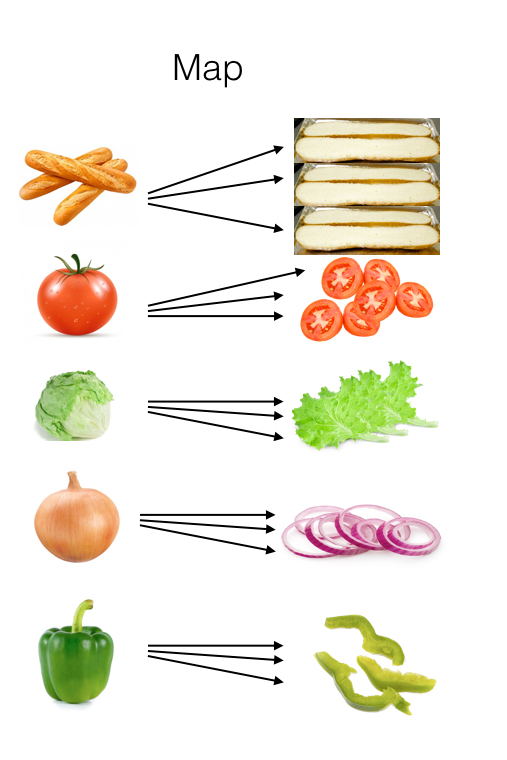
\includegraphics[width=.5\textwidth,height=.7\textheight]{./Figures/chapter-02/map-reduce-map-side.jpeg}
	\end{figure}			
	\footnotetext[1]{{\tiny This example taken from  \href{https://reberhardt.com/cs110/summer-2018/lecture-notes/lecture-14/}{https://reberhardt.com/cs110/summer-2018/lecture-notes/lecture-14/}	} }
\end{frame}
%%%%%%%%%%%%%%%%%%%%%%%%%%%%%%%%%%%%%%%%%%%%%%%%%%%%%%
\begin{frame}
	\frametitle{Shuffle/Group}
	We will organise and group the processed ingredients into piles, so that making a sandwich becomes easy.
		\begin{figure}
		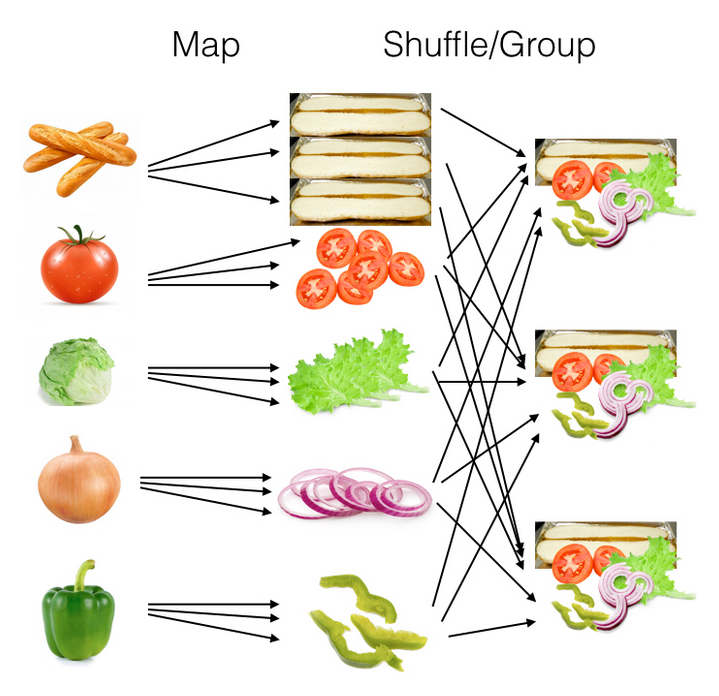
\includegraphics[width=.7\textwidth,height=.64\textheight]{./Figures/chapter-02/map-reduce-shuffle.png}
	\end{figure}			
	\footnotetext[1]{{\tiny This example taken from  \href{https://reberhardt.com/cs110/summer-2018/lecture-notes/lecture-14/}{https://reberhardt.com/cs110/summer-2018/lecture-notes/lecture-14/}	}} 
\end{frame}
%%%%%%%%%%%%%%%%%%%%%%%%%%%%%%%%%%%%%%%%%%%%%%%%%%%%%%
\begin{frame}
	\frametitle{Reduce}
	we’ll combine the ingredients into a sandwich
	\begin{figure}
		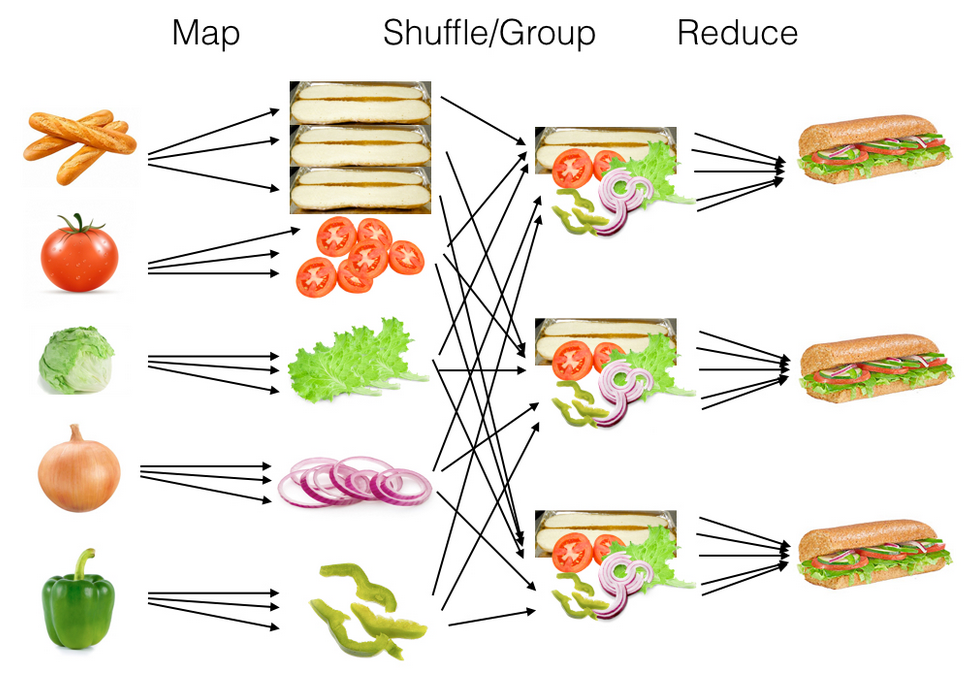
\includegraphics[width=.96\textwidth,height=.7\textheight]{./Figures/chapter-02/map-reduce-reduce-side.png}
	\end{figure}			
	\footnotetext[1]{ {\tiny This example taken from  \href{https://reberhardt.com/cs110/summer-2018/lecture-notes/lecture-14/}{https://reberhardt.com/cs110/summer-2018/lecture-notes/lecture-14/}	}} 
\end{frame}


%%%%%%%%%%%%%%%%%%%%%%%%%%%%%%%%%%%%%%%%%%%%%%%%%%%%%%
\begin{frame}[plain,c]
	\frametitle{Case Study Example 2}
	\begin{figure}
		\centering
		


\tikzset{every picture/.style={line width=0.75pt}} %set default line width to 0.75pt        

\begin{tikzpicture}[x=0.65pt,y=0.65pt,yscale=-1,xscale=1]
	%uncomment if require: \path (0,221); %set diagram left start at 0, and has height of 221
	
	
	%Shape: Rectangle [id:dp3221278753230701] 
	\draw [color=offred]  (2,60) -- (111,60) -- (111,90) -- (2,90) -- cycle ;
	%Shape: Rectangle [id:dp1271633566749788] 
	\draw [color=offred]  (2,140) -- (111,140) -- (111,170) -- (2,170) -- cycle ;
	%Curve Lines [id:da7576806433421945] 
	\draw  [line width=0.75,color=offwhite]  (112.42,59) .. controls (125,77.7) and (100.24,107.85) .. (128.62,109.05) ;

	%Curve Lines [id:da7014275949258858] 
	\draw [line width=0.75,color=offwhite]   (112,161.08) .. controls (125,137.56) and (97.32,110.2) .. (128.44,109.12) ;
	\draw [line width=0.75,color=offwhite] [shift={(130.42,109.08)}, rotate = 180] [color=offwhite  ][line width=0.75]    (10.93,-3.29) .. controls (6.95,-1.4) and (3.31,-0.3) .. (0,0) .. controls (3.31,0.3) and (6.95,1.4) .. (10.93,3.29)   ;
	%Rounded Rect [id:dp8577127496471914] 
	\draw   [color=offpurple] (131,103.47) .. controls (131,101.05) and (132.96,99.08) .. (135.38,99.08) -- (166.03,99.08) .. controls (168.45,99.08) and (170.42,101.05) .. (170.42,103.47) -- (170.42,116.62) .. controls (170.42,119.04) and (168.45,121) .. (166.03,121) -- (135.38,121) .. controls (132.96,121) and (131,119.04) .. (131,116.62) -- cycle ;
	%Rounded Rect [id:dp30434364847793793] 
	%%SPLIT 1
	\draw   [color={rgb, 255:red, 74; green, 144; blue, 226 }] 	(200,60) -- (250,60) -- (250,90) -- (200,90) -- cycle ;
	%Rounded Rect [id:dp4147495296848157] 
	%%SPLIT2
	
	\draw    [color={rgb, 255:red, 74; green, 144; blue, 226 }]  	(200,140) -- (250,140) -- (250,170) -- (200,170) -- cycle ;
	
	
	%Shape: Parallelogram [id:dp48792900018844987] 
	%%MAP
	\draw  [color=offyellow] (290,55.58) -- (323,55.58) -- (309,84) -- (277,84) -- cycle ;
	%Shape: Parallelogram [id:dp15766656313302363] 
	\draw [color=offyellow]  (290,140) -- (323,140) -- (309,166) -- (277,166) -- cycle ;
	
	%Straight Lines [id:da44147302793163634] 
	\draw  [line width=0.75,color=offwhite]  (251,70.79) -- (276,70.6) ;
	\draw  [line width=0.75,color=offwhite][shift={(280,70.58)}, rotate = 539.53] [color=offwhite  ][line width=0.75]    (10.93,-3.29) .. controls (6.95,-1.4) and (3.31,-0.3) .. (0,0) .. controls (3.31,0.3) and (6.95,1.4) .. (10.93,3.29)   ;
	
	
	%Straight Lines [id:da9443785238686285] 
	\draw  [line width=0.75,color=offwhite]  (251,151.79) -- (276,151.6) ;
	\draw [line width=0.75,color=offwhite] [shift={(278.42,151.58)}, rotate = 539.56] [color=offwhite  ][line width=0.75]    (10.93,-3.29) .. controls (6.95,-1.4) and (3.31,-0.3) .. (0,0) .. controls (3.31,0.3) and (6.95,1.4) .. (10.93,3.29)   ;
	%Shape: Rectangle [id:dp016273691107661636] 
	\draw [color={rgb, 255:red, 70; green, 155; blue, 36 }]  (342,47.58) -- (390,47.58) -- (390,106.58) -- (343,106.58) -- cycle ;
	%Straight Lines [id:da747872157663686] 
	\draw  [line width=0.75,color=offwhite]  (317,70) -- (338,70) ;
	\draw  [line width=0.75,color=offwhite] [shift={(340,70.58)}, rotate = 539.53] [color=offwhite  ][line width=0.75]    (10.93,-3.29) .. controls (6.95,-1.4) and (3.31,-0.3) .. (0,0) .. controls (3.31,0.3) and (6.95,1.4) .. (10.93,3.29)   ;
	%Straight Lines [id:da29503611504052674] 
	\draw  [line width=0.75,color=offwhite]  (317,156) -- (338,156) ;
\draw [line width=0.75,color=offwhite] [shift={(340.42,156.58)}, rotate = 539.53] [color=offwhite  ][line width=0.75]    (10.93,-3.29) .. controls (6.95,-1.4) and (3.31,-0.3) .. (0,0) .. controls (3.31,0.3) and (6.95,1.4) .. (10.93,3.29)   ;
	%Shape: Rectangle [id:dp4945355441436542] 
	%output
	\draw [color={rgb, 255:red, 70; green, 155; blue, 36 }]  (342,121) -- (390,121) -- (390,182.58) -- (343,182.58) -- cycle ;
	%Shape: Rectangle [id:dp7486542282421536] 
	%% outer box
	\draw   (188,20.58) -- (398.42,20.58) -- (398.42,110.58) -- (188,110.58) -- cycle ;
	%Shape: Rectangle [id:dp06285129437676396] 
	%%outerbox
	\draw   (188,110.58) -- (398.42,110.58) -- (398.42,200.58) -- (188,200.58) -- cycle ;
	%Rounded Rect [id:dp7025642442655686] 
	\draw   (414.42,98.18) .. controls (414.42,94.54) and (417.37,91.58) .. (421.02,91.58) -- (444.82,91.58) .. controls (448.46,91.58) and (451.42,94.54) .. (451.42,98.18) -- (451.42,117.98) .. controls (451.42,121.63) and (448.46,124.58) .. (444.82,124.58) -- (421.02,124.58) .. controls (417.37,124.58) and (414.42,121.63) .. (414.42,117.98) -- cycle ;
	%Shape: Rectangle [id:dp7889635565295128] 
	%% outer box
	\draw   (468.42,19.58) -- (670.42,19.58) -- (670.42,110.58) -- (468.42,110.58) -- cycle ;
	%Shape: Rectangle [id:dp8905165615601378] 
	%% outer box
	\draw   (468.42,110.58) -- (670.42,110.58) -- (670.42,200.58) -- (468.42,200.58) -- cycle ;
	%Shape: Rectangle [id:dp38010158785945036] 
	%input
	\draw [color={rgb, 255:red, 74; green, 144; blue, 226 } ]  (471,39.58) -- (523.42,39.58) -- (523.42,100.58) -- (471,100.58) -- cycle ;
	%Shape: Rectangle [id:dp7112194600890194] 
	%input
	\draw  [color={rgb, 255:red, 74; green, 144; blue, 226 } ] (471,127) -- (528.42,127) -- (528.42,187.58) -- (471,187.58) -- cycle ;
	
	%Shape: Parallelogram [id:dp8560234333811613] 
	\draw [color=offpink]  (555,53.58) -- (593,53.58) -- (580,82) -- (544,82) -- cycle ;
	%Shape: Parallelogram [id:dp03185670047818545] 
	\draw [color=offpink]  (555,132.58) -- (593,132.58) -- (580,161) -- (544,161) -- cycle ;
	
	
	%Shape: Rectangle [id:dp7083827174523002] 
	%output
	\draw [color={rgb, 255:red, 70; green, 155; blue, 36 }]  (610,36.58) -- (660,36.58) -- (660,96.58) -- (610,96.58) -- cycle ;
	%Shape: Rectangle [id:dp1906987565798669] 
	%output
	\draw [color={rgb, 255:red, 70; green, 155; blue, 36 }]  (610,130.58) -- (660,130.58) -- (660,180.58) -- (610,180.58) -- cycle ;
	
	%Straight Lines [id:da49186429007848953] 
	\draw  [line width=0.75,color=offwhite]  (523.21,69.79) -- (546.42,69.6) ;
	\draw [line width=0.75,color=offwhite] [shift={(548.42,69.58)}, rotate = 539.53] [color=offwhite  ][line width=0.75]    (10.93,-3.29) .. controls (6.95,-1.4) and (3.31,-0.3) .. (0,0) .. controls (3.31,0.3) and (6.95,1.4) .. (10.93,3.29)   ;
	%Straight Lines [id:da9429141358329266] 
	\draw  [line width=0.75,color=offwhite]  (583.21,67.79) -- (603.42,67.6) ;
	\draw [line width=0.75,color=offwhite] [shift={(605.42,67.58)}, rotate = 539.46] [color=offwhite  ][line width=0.75]    (10.93,-3.29) .. controls (6.95,-1.4) and (3.31,-0.3) .. (0,0) .. controls (3.31,0.3) and (6.95,1.4) .. (10.93,3.29)   ;
	%Straight Lines [id:da955760701625054] 
	\draw [line width=0.75,color=offwhite]   (586.21,146.79) -- (606.42,146.6) ;
	\draw [line width=0.75,color=offwhite] [shift={(608.42,146.58)}, rotate = 539.46] [color=offwhite  ][line width=0.75]    (10.93,-3.29) .. controls (6.95,-1.4) and (3.31,-0.3) .. (0,0) .. controls (3.31,0.3) and (6.95,1.4) .. (10.93,3.29)   ;
	%Straight Lines [id:da4689003855145568] 
	\draw [line width=0.75,color=offwhite]   (528.21,147.79) -- (546.42,147.6) ;
	\draw [line width=0.75,color=offwhite] [shift={(548.42,147.58)}, rotate = 539.4100000000001] [color=offwhite  ][line width=0.75]    (10.93,-3.29) .. controls (6.95,-1.4) and (3.31,-0.3) .. (0,0) .. controls (3.31,0.3) and (6.95,1.4) .. (10.93,3.29)   ;
	%Curve Lines [id:da21391955631880766] 
	\draw [line width=0.75,color=offwhite]   (454,108) .. controls (469.19,89.86) and (442.25,98.32) .. (466.28,70.86) ;
	\draw [line width=0.75,color=offwhite] [shift={(467.42,69.58)}, rotate = 491.88] [color=offwhite  ][line width=0.75]    (10.93,-3.29) .. controls (6.95,-1.4) and (3.31,-0.3) .. (0,0) .. controls (3.31,0.3) and (6.95,1.4) .. (10.93,3.29)   ;
	%Curve Lines [id:da1946353683290437] 
	\draw [line width=0.75,color=offwhite]   (454,108) .. controls (464.9,117.15) and (454.45,140.36) .. (463.94,148.53) ;
	\draw [line width=0.75,color=offwhite] [shift={(465.42,149.58)}, rotate = 210.26] [color=offwhite  ][line width=0.75]    (10.93,-3.29) .. controls (6.95,-1.4) and (3.31,-0.3) .. (0,0) .. controls (3.31,0.3) and (6.95,1.4) .. (10.93,3.29)   ;
	%Curve Lines [id:da6948926407425784] 
	\draw [line width=0.75,color=offwhite]   (398,68) .. controls (408,91.6) and (400.11,103.6) .. (413.61,110.72) ;
	\draw [line width=0.75,color=offwhite] [shift={(415.42,111.58)}, rotate = 203.63] [color=offwhite  ][line width=0.75]    (10.93,-3.29) .. controls (6.95,-1.4) and (3.31,-0.3) .. (0,0) .. controls (3.31,0.3) and (6.95,1.4) .. (10.93,3.29)   ;
	%Curve Lines [id:da5460745178214813] 
	\draw  [line width=0.75,color=offwhite]  (398.42,138.58) .. controls (413.22,124.74) and (399.6,114.44) .. (413.53,111.86) ;
	\draw  [line width=0.75,color=offwhite] [shift={(415.42,111.58)}, rotate = 533.29] [color=offwhite  ][line width=0.75]    (10.93,-3.29) .. controls (6.95,-1.4) and (3.31,-0.3) .. (0,0) .. controls (3.31,0.3) and (6.95,1.4) .. (10.93,3.29)   ;
	%Curve Lines [id:da3401941808176002] 
	\draw  [line width=0.75,color=offwhite]  (172,100) .. controls (180.25,88.81) and (159.28,65.54) .. (186.68,65.55) ;
	\draw [line width=0.75,color=offwhite] [shift={(188.42,65.58)}, rotate = 181.91] [color=offwhite  ][line width=0.75]    (10.93,-3.29) .. controls (6.95,-1.4) and (3.31,-0.3) .. (0,0) .. controls (3.31,0.3) and (6.95,1.4) .. (10.93,3.29)   ;
	%Curve Lines [id:da46994249585601144] 
	\draw  [line width=0.75,color=offwhite]  (172,100) .. controls (180.25,109.39) and (159.28,133.59) .. (185.74,135.49) ;
	\draw [line width=0.75,color=offwhite] [shift={(187.42,135.58)}, rotate = 181.97] [color=offwhite ][line width=0.75]    (10.93,-3.29) .. controls (6.95,-1.4) and (3.31,-0.3) .. (0,0) .. controls (3.31,0.3) and (6.95,1.4) .. (10.93,3.29)   ;
	
	% Text Node
	\draw (4,67) node [anchor=north west][inner sep=0.75pt]  [font=\scriptsize] [align=left,color=offred] {The cat came back};
	% Text Node
	\draw (41,90) node [anchor=north west][inner sep=0.75pt]  [font=\scriptsize] [align=left,color=offred] {split-1};
	% Text Node
	\draw (4,149) node [anchor=north west][inner sep=0.75pt]  [font=\scriptsize] [align=left,color=offred] {The very next day};
	% Text Node
	\draw (41,174) node [anchor=north west][inner sep=0.75pt]  [font=\scriptsize] [align=left,color=offred] {split-2};
	
	
	% Text Node
	\draw (133,102.08) node [anchor=north west][inner sep=0.75pt]   [align=left,color=offpurple] {{\scriptsize S \% n}};
	
	% Text Node
	\draw (205,66) node [anchor=north west][inner sep=0.75pt]  [font=\scriptsize,color=offred] [align=left] {split-1};
	% Text Node
	\draw (205,146) node [anchor=north west][inner sep=0.75pt]  [font=\scriptsize,color=offred] [align=left] {split-2};
	
	% Text Node
	\draw (285,65) node [anchor=north west][inner sep=0.75pt]  [font=\scriptsize] [align=left,color=offyellow] {map};
	% Text Node
	\draw (285,146) node [anchor=north west][inner sep=0.75pt]  [font=\scriptsize] [align=left,color=offyellow] {map};
	
	% Text Node
	\draw (270,98) node [anchor=north west][inner sep=0.75pt]  [font=\scriptsize] [align=left,color=offgreen2] {Node 1};
	% Text Node
	\draw (270,112) node [anchor=north west][inner sep=0.75pt]  [font=\scriptsize] [align=left,color=offgreen2] {Node 2};
	
	% Text Node
	\draw (342,50.58) node [anchor=north west][inner sep=0.75pt]  [font=\scriptsize] [align=left,color=offyellow] {(The,1) \\(cat,1)\\(came,1) \\(back,1)};
	% Text Node
	\draw (341,124) node [anchor=north west][inner sep=0.75pt]  [font=\scriptsize] [align=left,color=offyellow] {(The,1) \\(very,1)\\(next,1) \\(day,1)};
	
	% Text Node
	\draw (205,36) node [anchor=north west][inner sep=0.75pt]  [font=\scriptsize] [align=left,color={rgb, 255:red, 74; green, 144; blue, 226 } ] {input};
	% Text Node
	\draw (205,185.58) node [anchor=north west][inner sep=0.75pt]  [font=\scriptsize] [align=left,color={rgb, 255:red, 74; green, 144; blue, 226 } ] {input};
	
	% Text Node
	\draw (340,34) node [anchor=north west][inner sep=0.75pt]  [font=\scriptsize] [align=left,color={rgb, 255:red, 70; green, 155; blue, 36 }] {output};
	% Text Node
	\draw (340,186) node [anchor=north west][inner sep=0.75pt]  [font=\scriptsize] [align=left,color={rgb, 255:red, 70; green, 155; blue, 36 }] {output};

	% Text Node
	\draw (416,95) node [anchor=north west][inner sep=0.75pt]  [font=\tiny] [align=left] {Shuffle \\\& Soft};
	% Text Node
	
	
	\draw (470,42.58) node [anchor=north west][inner sep=0.75pt]  [font=\scriptsize] [align=left,color=offyellow] {(back,1)\\(cat,1)\\(came,1)\\(day,1)};
	% Text Node
	\draw (470,130) node [anchor=north west][inner sep=0.75pt]  [font=\scriptsize] [align=left,color=offyellow ] {(The,\{1,1\})\\(next,1)\\(very,1)};
	
	
	
	% Text Node
	\draw (551,64) node [anchor=north west][inner sep=0.75pt]  [font=\scriptsize] [align=left,color=offpink] {count};
	% Text Node
	\draw (551,142) node [anchor=north west][inner sep=0.75pt]  [font=\scriptsize] [align=left,color=offpink] {count};
	
	
	% Text Node
	\draw (610,39.58) node [anchor=north west][inner sep=0.75pt]  [font=\scriptsize] [align=left,color=offpink] {(back,1) \\(cat,1)\\(came,1)\\(day,1)};
	% Text Node
	\draw (610,132) node [anchor=north west][inner sep=0.75pt]  [font=\scriptsize] [align=left,color=offpink] {(The,2)\\(next,1)\\(very,1)};
	
	% Text Node
	\draw (286,184.58) node [anchor=north west][inner sep=0.75pt]  [font=\scriptsize] [align=left,color=offyellow] {fn};
	% Text Node
	\draw (286,34.58) node [anchor=north west][inner sep=0.75pt]  [font=\scriptsize] [align=left,color=offyellow] {fn};
	
	% Text Node
	\draw (552.22,112.58) node [anchor=north west][inner sep=0.75pt]  [font=\scriptsize] [align=left,color=offgreen2] {Node 2};
	% Text Node
	\draw (552.22,97.58) node [anchor=north west][inner sep=0.75pt]  [font=\scriptsize] [align=left,color=offgreen2] {Node 1};
	
	% Text Node
	\draw (610,24) node [anchor=north west][inner sep=0.75pt]  [font=\scriptsize] [align=left,color={rgb, 255:red, 70; green, 155; blue, 36 }] {output};
	% Text Node
	\draw (610,182) node [anchor=north west][inner sep=0.75pt]  [font=\scriptsize] [align=left,color={rgb, 255:red, 70; green, 155; blue, 36 }] {output};
	
	% Text Node
	\draw (560,186.33) node [anchor=north west][inner sep=0.75pt]  [font=\scriptsize] [align=left,color=offpink] {fn};
	% Text Node
	\draw (560,26.58) node [anchor=north west][inner sep=0.75pt]  [font=\scriptsize] [align=left,color=offpink] {fn};
	
	% Text Node
	\draw (470,27) node [anchor=north west][inner sep=0.75pt]  [font=\scriptsize] [align=left,color={rgb, 255:red, 74; green, 144; blue, 226 } ] {input};
	% Text Node
	\draw (470,188) node [anchor=north west][inner sep=0.75pt]  [font=\scriptsize] [align=left,color={rgb, 255:red, 74; green, 144; blue, 226 } ] {input};
	
	
	\draw (520.22,208) node [anchor=north west][inner sep=0.75pt]  [font=\footnotesize] [align=left] {Reduce side};
	\draw (260,208) node [anchor=north west][inner sep=0.75pt]  [font=\footnotesize] [align=left] {Map side};
	
\end{tikzpicture}

	\end{figure}
	
\end{frame}


\subsection{Introduction To Hadoop}

\begin{frame}[c]{ }
	\centering     
	
	\textcolor{offgreen}{ \large Previous video recap!}
\end{frame}



%%%%%%%%%%%%%%%%%%%%%%%%%%%%%%%%%%%%%%%%%%%%%%%%%%%%%%
\begin{frame}
	\frametitle{Lecture Objectives }
	\begin{itemize}  [<+->]
		\item Why do we need Hadoop?
		\item Hadoop Distributed File System (HDFS) concepts.
		\item Go dive into MapReduce.
		\item Hadoop architecture and its echosystems.
		\item How does Hadoop store, distribute, and process the data?

		
	\end{itemize}
\end{frame}
%%%%%%%%%%%%%%%%%%%%%%%%%%%%%%%%%%%%%%%%%%%%%%%%%%%%%%
\begin{frame}[c]{ }
	\frametitle{Introduction to Hadoop }
	\begin{itemize}  [<+->]
	\item Apache Hadoop's MapReduce and HDFS components were inspired by Google papers on MapReduce and Google File System
	
\end{itemize}
	\footnotetext[1]{From Wikipedia  \href{https://en.wikipedia.org/wiki/Apache_Hadoop}{https://en.wikipedia.org/wiki/Apache_Hadoop}	} 
	\footnotetext[2]{Google File System  \href{http://static.googleusercontent.com/media/research.google.com/en//archive/gfs-sosp2003.pdf}{http://static.googleusercontent.com/media/research.google.com/en//archive/gfs-sosp2003.pdf}	} 
	
	\footnotetext[3]{MapReduce: Simplifed Data Processing on Large Clusters \href{https://static.googleusercontent.com/media/research.google.com/en//archive/mapreduce-osdi04.pdf}{https://static.googleusercontent.com/media/research.google.com/en//archive/mapreduce-osdi04.pdf}	} 
	
\end{frame}

%%%%%%%%%%%%%%%%%%%%%%%%%%%%%%%%%%%%%%%%%%%%%%%%%%%%%%
\begin{frame}[c]{ }
		\frametitle{Introduction to Hadoop }
	\centering     
	
	\textcolor{offgreen}{ \large Is it already dead?}
\end{frame}
%%%%%%%%%%%%%%%%%%%%%%%%%%%%%%%%%%%%%%%%%%%%%%%%%%%%%%
\begin{frame}
	\frametitle{What is Hadoop? }
	\begin{itemize}  [<+->]
		\item A distributed software framework to store, process, and analzing "Large Scale of Data AKA. Big Data"
		\item It is open source!
		\item It runs on commodity (standard) hardware.
		\item Hadoop architecture and its echosystems.		
	\end{itemize}
\end{frame}
%%%%%%%%%%%%%%%%%%%%%%%%%%%%%%%%%%%%%%%%%%%%%%%%%%%%%%
\begin{frame}
	\frametitle{Hadoop Core Components }
	\begin{itemize}  [<+->]
		
		\item Hadoop HDFS: Data Storage Layer (File System).
		\item Hadoop MapReduce: The processing engine (compute paradigm) in Hadoop.
		\item Hadoop YARN: The resource manager in Hadoop.
		
	\end{itemize}
\end{frame}
%%%%%%%%%%%%%%%%%%%%%%%%%%%%%%%%%%%%%%%%%%%%%%%%%%%%%%
\begin{frame}[c]{ }
	\frametitle{Introduction to Hadoop }
	\centering     
	
	\textcolor{offgreen}{ \large What are the alternatives?}
\end{frame}
%%%%%%%%%%%%%%%%%%%%%%%%%%%%%%%%%%%%%%%%%%%%%%%%%%%%%%
\begin{frame}
	\frametitle{Hadoop Core Components }
	\begin{itemize}  
		
		\item \sout{Hadoop HDFS} \textcolor{offyellow}{S3/GFS}:  Data Storage Layer (File System).
		\item \sout{Hadoop MapReduce} \textcolor{offyellow}{Spark/Flink}: The processing engine (compute paradigm) in Hadoop.
		\item \sout{Hadoop YARN} \textcolor{offyellow}{Kubernetes}: The resource manager in Hadoop.
		% \textcolor{brown}{
	\end{itemize}
\end{frame}
%%%%%%%%%%%%%%%%%%%%%%%%%%%%%%%%%%%%%%%%%%%%%%%%%%%%%%
\begin{frame}[c]{ }
	\frametitle{Introduction to Hadoop }
	\centering     
	
	\textcolor{offgreen}{ \large Can we use these alternatives on prem?}
\end{frame}
%%%%%%%%%%%%%%%%%%%%%%%%%%%%%%%%%%%%%%%%%%%%%%%%%%%%%%
\begin{frame}
	\frametitle{Hadoop Echosystem }
	\begin{figure}
	\centering
	


\tikzset{every picture/.style={line width=0.75pt}} %set default line width to 0.75pt        


\def \xOne {12}
\def \xTwo {522}
\def \yOne {165}
\def \yTwo {195}
\def \yOneDelta {40}
\def \yTwoDelta {35}
\def \yTwoShift {5}

\def \hcboxXOne{20}
\def \hcboxXTwo{110}
\def \hcboxYOne{25}
\def \hcboxYTwo{50}
\def \hcboxXShift{100}

\def \dsXOne{60}
\def \dsXTwo{190}
\def \dsYOne{130}
\def \dsYTwo{155}
\def \dsXShift{270}

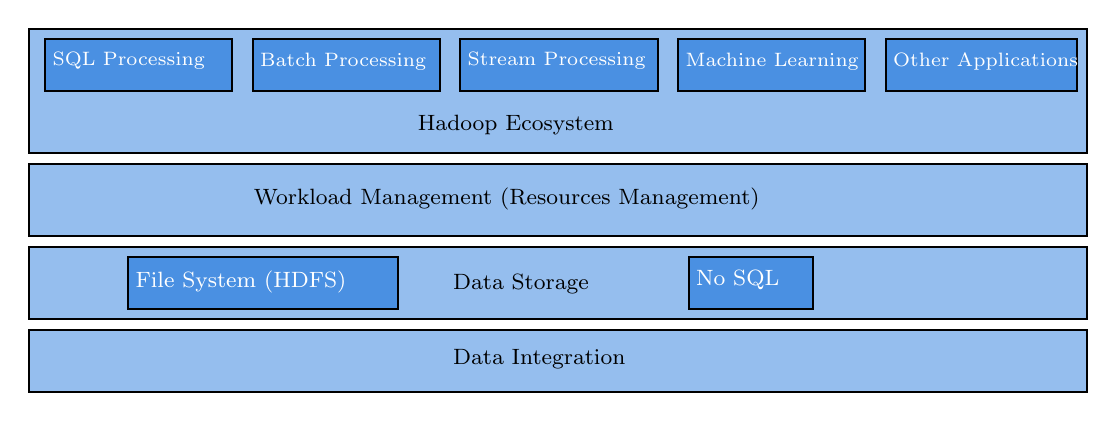
\begin{tikzpicture}[x=0.75pt,y=0.75pt,yscale=-1,xscale=1]

	
	%Shape: Rectangle [id:dp9526398227547324] 
	\draw [fill={rgb, 255:red, 74; green, 144; blue, 226 }  ,fill opacity=0.59 ] (\xOne,\yOne) -- (\xTwo,\yOne) -- (\xTwo,\yTwo) -- (\xOne,\yTwo) -- cycle ;
	%Shape: Rectangle [id:dp34591779607428674] 
	\draw  [fill={rgb, 255:red, 74; green, 144; blue, 226 }  ,fill opacity=0.59 ] (\xOne,\yOne-\yOneDelta) -- (\xTwo,\yOne-\yOneDelta) -- (\xTwo,\yTwo-\yTwoDelta) -- (\xOne,\yTwo-\yTwoDelta) -- cycle ;

	%Shape: Rectangle [id:dp45758690857887285] 
	\draw [fill={rgb, 255:red, 74; green, 144; blue, 226 }  ,fill opacity=0.59 ] (\xOne,\yOne-\yOneDelta*2) -- (\xTwo,\yOne-\yOneDelta*2) -- (\xTwo,\yTwo-\yTwoDelta*2 - \yTwoShift) -- (\xOne,\yTwo-\yTwoDelta*2 - \yTwoShift) -- cycle ;
	%Shape: Rectangle [id:dp7537784714823494] 
	\draw [fill={rgb, 255:red, 74; green, 144; blue, 226 }  ,fill opacity=0.59 ] (\xOne,\yOne-\yOneDelta*3-25) -- (\xTwo,\yOne-\yOneDelta*3-25) -- (\xTwo,\yTwo-\yTwoDelta*3 -\yTwoShift*2) -- (\xOne,\yTwo-\yTwoDelta*3 -\yTwoShift*2) -- cycle ;
	
	
	%Rounded Rect [id:dp9146242593539052] 
	\draw  [fill={rgb, 255:red, 74; green, 144; blue, 226 }  ,fill opacity=1 ] (\dsXOne,\dsYOne) -- (\dsXTwo,\dsYOne) -- (\dsXTwo,\dsYTwo) -- (\dsXOne,\dsYTwo) -- cycle ;
	%Rounded Rect [id:dp07383423201361416] 
	\draw  [fill={rgb, 255:red, 74; green, 144; blue, 226 }  ,fill opacity=1 ] (\dsXOne+\dsXShift,\dsYOne) -- (\dsXTwo-70+\dsXShift,\dsYOne) -- (\dsXTwo+\dsXShift-70,\dsYTwo) -- (\dsXOne+\dsXShift,\dsYTwo) -- cycle ;
	
	
	
	
	%Rounded Rect [id:dp8181874793090042] 
	\draw  [fill={rgb, 255:red, 74; green, 144; blue, 226 }  ,fill opacity=1 ] (\hcboxXOne,\hcboxYOne) -- (\hcboxXTwo,\hcboxYOne) -- (\hcboxXTwo,\hcboxYTwo) -- (\hcboxXOne,\hcboxYTwo) -- cycle ;
	%Rounded Rect [id:dp9716087561496145] 
	\draw  [fill={rgb, 255:red, 74; green, 144; blue, 226 }  ,fill opacity=1 ] (\hcboxXOne+\hcboxXShift,\hcboxYOne) -- (\hcboxXTwo+\hcboxXShift,\hcboxYOne) -- (\hcboxXTwo+\hcboxXShift,\hcboxYTwo) -- (\hcboxXOne+\hcboxXShift,\hcboxYTwo) -- cycle ;
	%Rounded Rect [id:dp6064393858129398] 
	\draw  [fill={rgb, 255:red, 74; green, 144; blue, 226 }  ,fill opacity=1 ] (\hcboxXOne+\hcboxXShift*2,\hcboxYOne) -- (\hcboxXTwo+\hcboxXShift*2+5,\hcboxYOne) -- (\hcboxXTwo+\hcboxXShift*2+5,\hcboxYTwo) -- (\hcboxXOne+\hcboxXShift*2,\hcboxYTwo) -- cycle ;
	%Rounded Rect [id:dp9339323209047331] 
	\draw  [fill={rgb, 255:red, 74; green, 144; blue, 226 }  ,fill opacity=1 ] (\hcboxXOne+\hcboxXShift*3+5,\hcboxYOne) -- (\hcboxXTwo+\hcboxXShift*3+5,\hcboxYOne) -- (\hcboxXTwo+\hcboxXShift*3+5,\hcboxYTwo) -- (\hcboxXOne+\hcboxXShift*3+5,\hcboxYTwo) -- cycle ;
	%Rounded Rect [id:dp5657335982682512] 
	\draw  [fill={rgb, 255:red, 74; green, 144; blue, 226 }  ,fill opacity=1 ] (\hcboxXOne+\hcboxXShift*4+5,\hcboxYOne) -- (\hcboxXTwo+\hcboxXShift*4+7,\hcboxYOne) -- (\hcboxXTwo+\hcboxXShift*4+7,\hcboxYTwo) -- (\hcboxXOne+\hcboxXShift*4+5,\hcboxYTwo) -- cycle ;

	% Text Node
	\draw (215,173) node [anchor=north west][inner sep=0.75pt]  [font=\footnotesize] [align=left] {Data Integration};
	% Text Node
	\draw (\dsXOne+2,\dsYOne+5) node [anchor=north west][inner sep=0.75pt]  [font=\footnotesize,color={rgb, 255:red, 255; green, 255; blue, 255 }  ,opacity=1 ] [align=left] {File System (HDFS)};
	% Text Node
	\draw (\dsXOne+\dsXShift+2,\dsYOne+5) node [anchor=north west][inner sep=0.75pt]  [font=\footnotesize,color={rgb, 255:red, 255; green, 255; blue, 255 }  ,opacity=1 ] [align=left] {No SQL};

	% Text Node
	\draw (215,137) node [anchor=north west][inner sep=0.75pt]  [font=\footnotesize] [align=left] {Data Storage};
	% Text Node
	\draw (119,95) node [anchor=north west][inner sep=0.75pt]  [font=\footnotesize] [align=left] {Workload Management (Resources Management)};
	% Text Node
	\draw (198,60) node [anchor=north west][inner sep=0.75pt]  [font=\footnotesize] [align=left] {Hadoop Ecosystem};
	
	% Text Node
	\draw (\hcboxXOne +2 ,\hcboxYOne +5) node [anchor=north west][inner sep=0.75pt]  [font={\scriptsize },color={rgb, 255:red, 255; green, 255; blue, 255 }  ,opacity=1 ] [align=left] {SQL Processing};
	% Text Node
	\draw (\hcboxXOne +2+\hcboxXShift,\hcboxYOne +5) node [anchor=north west][inner sep=0.75pt]  [font=\scriptsize,color={rgb, 255:red, 255; green, 255; blue, 255 }  ,opacity=1 ] [align=left] {Batch Processing};
	% Text Node
	\draw (\hcboxXOne +2+\hcboxXShift*2,\hcboxYOne +5) node [anchor=north west][inner sep=0.75pt]  [font=\scriptsize,color={rgb, 255:red, 255; green, 255; blue, 255 }  ,opacity=1 ] [align=left] {Stream Processing};
	% Text Node
	\draw (\hcboxXOne +7+\hcboxXShift*3,\hcboxYOne +5) node [anchor=north west][inner sep=0.75pt]  [font=\scriptsize,color={rgb, 255:red, 255; green, 255; blue, 255 }  ,opacity=1 ] [align=left] {Machine Learning};
	% Text Node
	\draw (\hcboxXOne +7+\hcboxXShift*4,\hcboxYOne +5) node [anchor=north west][inner sep=0.75pt]  [font=\scriptsize,color={rgb, 255:red, 255; green, 255; blue, 255 }  ,opacity=1 ] [align=left] {Other Applications};
	
	
\end{tikzpicture}
%%%%%%%%%%%%%%%%%%%%%%%%%%%%%%%%%%%%%%%%%%%%%%%%%%%%%%%%%%%%%%%%%%%%%%%%%%%
%%% Local Variables:
%%% mode: latex
%%% TeX-master: "../../main.tex"
% !TeX root = ../../main.tex
%%% TeX-engine: xetex
%%% End:

	\caption{Hadoop Architecture } \label{fig:DS3}
\end{figure}
\end{frame}
%%%%%%%%%%%%%%%%%%%%%%%%%%%%%%%%%%%%%%%%%%%%%%%%%%%%%%
\begin{frame}[c]{ }
	\frametitle{Hadoop Motivation }
	\centering     
	
	\textcolor{offgreen}{ \large Hadoop Motivation}
\end{frame}
%%%%%%%%%%%%%%%%%%%%%%%%%%%%%%%%%%%%%%%%%%%%%%%%%%%%%%
\begin{frame}[c]{ }
	\frametitle{Hadoop Motivation }
	Processing:
	\begin{itemize}  [<+->]
	
	\item Traditional Computation was depending on bigger computers to deal with bigger data.
	\item This method has a bottleneck in the computation (Moore's Law), but this couldn't keep up.
	\item The better solution requires more computers (distributed computing framework).
	
\end{itemize}
\end{frame}
%%%%%%%%%%%%%%%%%%%%%%%%%%%%%%%%%%%%%%%%%%%%%%%%%%%%%%
\begin{frame}[c]{ }
	\frametitle{Hadoop Motivation }
	Storage:
	\begin{itemize}  [<+->]
		
		\item Traditional Computation store the data in a central unit.
		\item Data was copied (moved) to the computation nodes, for example, IBM Data stage or Talend.
		\item The process of copying or moving the data was fine when we move a small amount of data, but the big data will cause lots of problems, especially in the network bandwidth, and data moving will be costly.
		
	\end{itemize}
\end{frame}

%%%%%%%%%%%%%%%%%%%%%%%%%%%%%%%%%%%%%%%%%%%%%%%%%%%%%%
\begin{frame}[c]{ }
	\frametitle{Requirements for The New Approach }
	
	
	\begin{itemize}  [<+->]
		\item [--] Fault Tolerance.
		\item [--] High Availability.
		\item [--] Reliability.
		\item [--] Scalability.
		\item [--] Consistency.
		\item [--] Data Locality.
		\item [--] Economic.
		
	\end{itemize}
\end{frame}
%%%%%%%%%%%%%%%%%%%%%%%%%%%%%%%%%%%%%%%%%%%%%%%%%%%%%%
\begin{frame}[c]{ }
	\frametitle{Requirements for The New Approach }
	Economic
	\begin{itemize}  [<+->]
		\item [--] {\footnotesize It uses commodity (Standard/Economic) hardware}.

	\end{itemize}
\end{frame}
%%%%%%%%%%%%%%%%%%%%%%%%%%%%%%%%%%%%%%%%%%%%%%%%%%%%%%
\begin{frame}[c]{ }
	\frametitle{Requirements for The New Approach }
	Data Locality
	\begin{itemize}  [<+->]
		\item [--] {\footnotesize It brings the program to the data rather than the data to the program. It runs the computation where the data reside.}		
		\item [--] {\footnotesize HDFS is strongly consistent.}		
	\end{itemize}
\end{frame}
%%%%%%%%%%%%%%%%%%%%%%%%%%%%%%%%%%%%%%%%%%%%%%%%%%%%%%
\begin{frame}[c]{ }
	\frametitle{Requirements for The New Approach }
	Fault Tolerance
	\begin{itemize}  [<+->]
		\item [--] {\footnotesize It is the property that enables a system to continue operating properly in the event of the failure of (or one or more faults within) some of its components}.
		\item [--] {\footnotesize The ability of maintaining functionality when portions of a system break down is referred to as graceful degradation}.
		\item [--] {\footnotesize A fault-tolerant design enables a system to continue its intended operation, possibly at a reduced level, rather than failing completely, when some part of the system fails.}
		
	\end{itemize}
	\footnotetext[1]{From Wikipedia  \href{https://en.wikipedia.org/wiki/Fault_tolerance}{https://en.wikipedia.org/wiki/Fault_tolerance}	} 
\end{frame}
%%%%%%%%%%%%%%%%%%%%%%%%%%%%%%%%%%%%%%%%%%%%%%%%%%%%%%
\begin{frame}[c]{ }
	\frametitle{Requirements for The New Approach }
	High Availability
	\begin{itemize}  [<+->]
		\item [--] {\footnotesize High availability (HA) is a characteristic of a system which aims to ensure an agreed level of operational performance, usually uptime, for a higher than normal period}.
		\item [--] {\footnotesize The availability of the cluster (system) to operate without any downtime despite any hardware failure. The data or the system should be available and accessed from any alternative way}.
		
	\end{itemize}
	\footnotetext[1]{From Wikipedia  \href{https://en.wikipedia.org/wiki/High_availability}{https://en.wikipedia.org/wiki/High_availability}	} 
\end{frame}

%%%%%%%%%%%%%%%%%%%%%%%%%%%%%%%%%%%%%%%%%%%%%%%%%%%%%%
\begin{frame}[c]{ }
	\frametitle{Requirements for The New Approach }
	Reliability
	\begin{itemize}  [<+->]
		\item [--] {\footnotesize The data reliably stored on the cluster of machine despite machine failures. }		
	\end{itemize}
\end{frame}
%%%%%%%%%%%%%%%%%%%%%%%%%%%%%%%%%%%%%%%%%%%%%%%%%%%%%%
\begin{frame}[c]{ }
	\frametitle{Requirements for The New Approach }
	Scalability
	\begin{itemize}  [<+->]
		\item [--] {\footnotesize The system must be highly scalable in both vertical and horizontal. This means we can add a new node to an existing cluster easily or add new hardware to an existing node.}		
	\end{itemize}
\end{frame}
%%%%%%%%%%%%%%%%%%%%%%%%%%%%%%%%%%%%%%%%%%%%%%%%%%%%%%
\begin{frame}[c]{ }
	\frametitle{Requirements for The New Approach }
	Consistency
	\begin{itemize}  [<+->]
		\item [--] {\footnotesize Any failure during the execution job shouldn't affect the outcome of the job.}		
		\item [--] {\footnotesize HDFS is strongly consistent.}		
	\end{itemize}
\end{frame}
%%%%%%%%%%%%%%%%%%%%%%%%%%%%%%%%%%%%%%%%%%%%%%%%%%%%%%
\begin{frame}[c]{ }
	\frametitle{Core Hadoop Concepts }
	\centering     
	
	\textcolor{offgreen}{ \large Hadoop Core Concepts}
\end{frame}
%%%%%%%%%%%%%%%%%%%%%%%%%%%%%%%%%%%%%%%%%%%%%%%%%%%%%%
\begin{frame}[c]{ }
	\frametitle{Hadoop Core Concepts }
	
	
	\begin{itemize}  [<+->]
		\item [--] Hadoop is scalable and fault-tolerant.
		\item [--] Hadoop replicates the data to increase the availability and reliability.
		\item [--] Hadoop brings the program to the data.
		\item [--] Applications are written in high-level code.
		\item [--] Hadoop reduces the data movement (shuffle) between the nodes.
		
	\end{itemize}
\end{frame}

%%%%%%%%%%%%%%%%%%%%%%%%%%%%%%%%%%%%%%%%%%%%%%%%%%%%%%
\begin{frame}[c]{ }
	\frametitle{Core Hadoop Concepts }
	\centering     
	
	\textcolor{offgreen}{ \large Hadoop Core Components}
\end{frame}
%%%%%%%%%%%%%%%%%%%%%%%%%%%%%%%%%%%%%%%%%%%%%%%%%%%%%%
\begin{frame}[c]{ }
	\frametitle{Hadoop Core Concepts }
	
	
	\begin{itemize}  [<+->]
		\item [--] HDFS.
		\item [--] Map-Reduce.
		\item [--] YARN.
		
	\end{itemize}
\end{frame}
%%%%%%%%%%%%%%%%%%%%%%%%%%%%%%%%%%%%%%%%%%%%%%%%%%%%%%
\begin{frame}[c]{ }
	\frametitle{HDFS }
	
	
	\begin{itemize}  [<+->]
		\item [--] HDFS responsible for storing the data on the hadoop cluster.
		\item [--] Data is split into blocks with configurable block size, for example 64MB, 128MB, 512MB.
		\item [--] Each data block is replicated and distributed across the cluster data node. This replication is configrable and by default three replica.
		\item [--] Each block is stored in three different nodes. It is recommended to have two nodes in the same rack and the third one in a different rack.
		
	\end{itemize}
\end{frame}
%%%%%%%%%%%%%%%%%%%%%%%%%%%%%%%%%%%%%%%%%%%%%%%%%%%%%%
\begin{frame}[c]{ }
	\frametitle{HDFS }
	
	
	\begin{itemize}  [<+->]
		\item [--] {\footnotesize HDFS is responsible for storing the data on the Hadoop cluster.}
		\item [--] {\footnotesize Data is split into blocks with configurable block size, for example, 64MB, 128MB, and 512MB.}
		\item [--] {\footnotesize Each data block is replicated and distributed across the cluster data node. This replication is configurable, and by default, three replica (folds).}
		\item [--] {\footnotesize Each block is stored in three different nodes. It is recommended to have two nodes in the same rack and the third one in a different rack.}
		\item [--] {\footnotesize A \textit{NameNode} keeps track of the location of the blocks and which blocks make up these files. These details known as \textit{metadata}.}
	\end{itemize}
\end{frame}
%%%%%%%%%%%%%%%%%%%%%%%%%%%%%%%%%%%%%%%%%%%%%%%%%%%%%%
\begin{frame}[c]{ }
	\frametitle{HDFS }
		\begin{figure}
		\centering
		


\tikzset{every picture/.style={line width=0.75pt}} %set default line width to 0.75pt        

\begin{tikzpicture}[x=0.6pt,y=0.6pt,yscale=-1,xscale=1]
%uncomment if require: \path (0,300); %set diagram left start at 0, and has height of 300

%Shape: Rectangle [id:dp893573566833787] 
\draw  [fill=MyGray  ,fill opacity=1 ] (3.17,163.17) -- (291.33,163.17) -- (291.33,294.5) -- (3.17,294.5) -- cycle ;
%Shape: Rectangle [id:dp46281852294984216] 
\draw  [fill=offpurple ,fill opacity=1 ] (8.33,170.33) -- (234.33,170.33) -- (234.33,271.33) -- (8.33,271.33) -- cycle ;
%Shape: Rectangle [id:dp6261320843201246] 
\draw   (10,62) -- (80,62) -- (80,102) -- (10,102) -- cycle ;
%Snip Single Corner Rect [id:dp12418640338729592] 
\draw  [fill=brown  ,fill opacity=1 ]  (211,61) -- (137,61) -- (123.33,47) -- (123.33,21) -- (211,21) -- cycle ;
%Snip Single Corner Rect [id:dp30064468613598183] 
\draw  [fill=brown  ,fill opacity=1 ]  (211,141) -- (137,141) -- (123.33,127) -- (123.33,101) -- (211,101) -- cycle ;
%Straight Lines [id:da7812791931414549] 
\draw  [->]  (81.33,82.33) -- (123,47) ;
%Straight Lines [id:da010110675330870511] 
\draw  [->]  (81.33,82.33) -- (123,127) ;
%Rounded Rect [id:dp35954418736480753] 
\draw  [fill=offgreen  ,fill opacity=1 ] (298,81.67) .. controls (298,52.03) and (322.03,28) .. (351.67,28) -- (603.67,28) .. controls (633.31,28) and (657.33,52.03) .. (657.33,81.67) -- (657.33,242.67) .. controls (657.33,272.31) and (633.31,296.33) .. (603.67,296.33) -- (351.67,296.33) .. controls (322.03,296.33) and (298,272.31) .. (298,242.67) -- cycle ;

%Shape: Rectangle [id:dp8687762741846744] 
\draw  [fill=ballblue  ,fill opacity=1 ] (327,55) -- (478.33,55) -- (478.33,276.33) -- (327,276.33) -- cycle ;
%Shape: Rectangle [id:dp7548707221284656] 
\draw  [fill=spirodiscoball  ,fill opacity=1 ] (489,55) -- (640.33,55) -- (640.33,276.33) -- (489,276.33) -- cycle ;

%Rounded Rect [id:dp00897404914951061] 
\draw  [fill={rgb, 255:red, 237; green, 227; blue, 227 }  ,fill opacity=1 ] (355,84) .. controls (355,79.58) and (358.58,76) .. (363,76) -- (439.33,76) .. controls (443.75,76) and (447.33,79.58) .. (447.33,84) -- (447.33,108) .. controls (447.33,112.42) and (443.75,116) .. (439.33,116) -- (363,116) .. controls (358.58,116) and (355,112.42) .. (355,108) -- cycle ;

%Rounded Rect [id:dp9790517680808902] 
\draw  [fill={rgb, 255:red, 237; green, 227; blue, 227 }  ,fill opacity=1 ]  (355,144) .. controls (355,139.58) and (358.58,136) .. (363,136) -- (439.33,136) .. controls (443.75,136) and (447.33,139.58) .. (447.33,144) -- (447.33,168) .. controls (447.33,172.42) and (443.75,176) .. (439.33,176) -- (363,176) .. controls (358.58,176) and (355,172.42) .. (355,168) -- cycle ;
%Rounded Rect [id:dp013627781761065716] 
\draw  [fill={rgb, 255:red, 237; green, 227; blue, 227 }  ,fill opacity=1 ] (356,204) .. controls (356,199.58) and (359.58,196) .. (364,196) -- (438.33,196) .. controls (442.75,196) and (446.33,199.58) .. (446.33,204) -- (446.33,228) .. controls (446.33,232.42) and (442.75,236) .. (438.33,236) -- (364,236) .. controls (359.58,236) and (356,232.42) .. (356,228) -- cycle ;
%Rounded Rect [id:dp8935666136526693] 
\draw  [fill={rgb, 255:red, 237; green, 227; blue, 227 }  ,fill opacity=1 ] (520,85) .. controls (520,80.58) and (523.58,77) .. (528,77) -- (601.33,77) .. controls (605.75,77) and (609.33,80.58) .. (609.33,85) -- (609.33,109) .. controls (609.33,113.42) and (605.75,117) .. (601.33,117) -- (528,117) .. controls (523.58,117) and (520,113.42) .. (520,109) -- cycle ;

\draw  [fill={rgb, 255:red, 237; green, 227; blue, 227 }  ,fill opacity=1 ] (520,145) .. controls (520,140.58) and (523.58,137) .. (528,137) -- (601.33,137) .. controls (605.75,137) and (609.33,140.58) .. (609.33,145) -- (609.33,169) .. controls (609.33,173.42) and (605.75,177) .. (601.33,177) -- (528,177) .. controls (523.58,177) and (520,173.42) .. (520,169) -- cycle ;

%Rounded Rect [id:dp24192848422071778] 
\draw  [fill={rgb, 255:red, 237; green, 227; blue, 227 }  ,fill opacity=1 ] (521,205) .. controls (521,200.58) and (524.58,197) .. (529,197) -- (601.33,197) .. controls (605.75,197) and (609.33,200.58) .. (609.33,205) -- (609.33,229) .. controls (609.33,233.42) and (605.75,237) .. (601.33,237) -- (529,237) .. controls (524.58,237) and (521,233.42) .. (521,229) -- cycle ;


%Shape: Circle [id:dp6662144240379807] 
%%file left panel
\draw[fill={rgb, 255:red, 74; green, 144; blue, 226 }, thick] (223,28) circle (.2 cm);
\draw (218,22) node [anchor=north west][inner sep=0.75pt]  [color=white  ,opacity=1 ]  [font=\scriptsize]  [align=left] {1};

\draw[fill={rgb, 255:red, 245; green, 166; blue, 35 }, thick] (223,52) circle (.2 cm);
\draw (218,46) node [anchor=north west][inner sep=0.75pt]  [color=black  ,opacity=1 ]  [font=\scriptsize]  [align=left] {2};

\draw[fill={rgb, 255:red, 139; green, 87; blue, 42 }, thick] (223,98) circle (.2 cm);
\draw (218,92) node [anchor=north west][inner sep=0.75pt]  [color=white  ,opacity=1 ]  [font=\scriptsize]  [align=left] {3};

\draw[fill={rgb, 255:red, 126; green, 211; blue, 33 }, thick] (223,122) circle (.2 cm);
\draw (218,116) node [anchor=north west][inner sep=0.75pt]  [color=black  ,opacity=1 ]  [font=\scriptsize]  [align=left] {4};

\draw[fill={rgb, 255:red, 208; green, 2; blue, 27 }, thick] (223,146) circle (.2 cm);
\draw (218,140) node [anchor=north west][inner sep=0.75pt]  [color=white  ,opacity=1 ]  [font=\scriptsize]  [align=left] {5};


\draw[fill={rgb, 255:red, 74; green, 144; blue, 226 }, thick] (365,102) circle (.2 cm);
\draw (360,96) node [anchor=north west][inner sep=0.75pt]  [color=white  ,opacity=1 ]  [font=\scriptsize]  [align=left] {1};

\draw[fill={rgb, 255:red, 245; green, 166; blue, 35 }, thick] (390,102) circle (.2 cm);
\draw (385,96) node [anchor=north west][inner sep=0.75pt]  [color=black  ,opacity=1 ]  [font=\scriptsize]  [align=left] {2};

\draw[fill={rgb, 255:red, 126; green, 211; blue, 33 }, thick] (415,102) circle (.2 cm);
\draw (410,96) node [anchor=north west][inner sep=0.75pt]  [color=black  ,opacity=1 ]  [font=\scriptsize]  [align=left] {3};


\draw[fill={rgb, 255:red, 74; green, 144; blue, 226 }, thick] (365,163) circle (.2 cm);
\draw (360,157) node [anchor=north west][inner sep=0.75pt]  [color=white  ,opacity=1 ]  [font=\scriptsize]  [align=left] {1};

\draw[fill={rgb, 255:red, 245; green, 166; blue, 35 }, thick] (390,163) circle (.2 cm);
\draw (385,157) node [anchor=north west][inner sep=0.75pt]  [color=black  ,opacity=1 ]  [font=\scriptsize]  [align=left] {2};

\draw[fill={rgb, 255:red, 208; green, 2; blue, 27 }, thick] (415,163) circle (.2 cm);
\draw (410,157) node [anchor=north west][inner sep=0.75pt]  [color=white  ,opacity=1 ]  [font=\scriptsize]  [align=left] {5};

\draw[fill={rgb, 255:red, 126; green, 211; blue, 33 }, thick] (365,224) circle (.2 cm);
\draw (360,218) node [anchor=north west][inner sep=0.75pt]  [color=black  ,opacity=1 ]  [font=\scriptsize]  [align=left] {1};

\draw[fill={rgb, 255:red, 139; green, 87; blue, 42 }, thick] (390,224) circle (.2 cm);
\draw (385,218) node [anchor=north west][inner sep=0.75pt]  [color=white  ,opacity=1 ]  [font=\scriptsize]  [align=left] {1};


\draw[fill={rgb, 255:red, 74; green, 144; blue, 226 }, thick] (530,102) circle (.2 cm);
\draw (525,96) node [anchor=north west][inner sep=0.75pt]  [color=white  ,opacity=1 ]  [font=\scriptsize]  [align=left] {1};

\draw[fill={rgb, 255:red, 139; green, 87; blue, 42 }, thick] (555,102) circle (.2 cm);
\draw (550,96) node [anchor=north west][inner sep=0.75pt]  [color=white  ,opacity=1 ]  [font=\scriptsize]  [align=left] {3};

\draw[fill={rgb, 255:red, 208; green, 2; blue, 27 }, thick] (580,102) circle (.2 cm);
\draw (575,96) node [anchor=north west][inner sep=0.75pt]  [color=white  ,opacity=1 ]  [font=\scriptsize]  [align=left] {5};


\draw[fill={rgb, 255:red, 245; green, 166; blue, 35 }, thick] (530,163) circle (.2 cm);
\draw (525,157) node [anchor=north west][inner sep=0.75pt]  [color=black  ,opacity=1 ]  [font=\scriptsize]  [align=left] {2};

\draw[fill={rgb, 255:red, 139; green, 87; blue, 42 }, thick] (555,163) circle (.2 cm);
\draw (550,157) node [anchor=north west][inner sep=0.75pt]  [color=white  ,opacity=1 ]  [font=\scriptsize]  [align=left] {3};


\draw[fill={rgb, 255:red, 126; green, 211; blue, 33 }, thick] (530,224) circle (.2 cm);
\draw (525,218) node [anchor=north west][inner sep=0.75pt]  [color=black  ,opacity=1 ]  [font=\scriptsize]  [align=left] {4};

\draw[fill={rgb, 255:red, 208; green, 2; blue, 27 }, thick] (555,224) circle (.2 cm);
\draw (550,218) node [anchor=north west][inner sep=0.75pt]  [color=white  ,opacity=1 ]  [font=\scriptsize]  [align=left] {5};



% Text Node
\draw (25,75) node [anchor=north west][inner sep=0.75pt]   [font=\scriptsize] [align=left] {client};
% Text Node
\draw (126,24) node [anchor=north west][inner sep=0.75pt]  [font=\scriptsize] [align=left] {/sales/\\20210521.csv};
% Text Node
\draw (126,104) node [anchor=north west][inner sep=0.75pt]  [font=\scriptsize] [align=left] {/sales/\\20210522.csv};
% Text Node
\draw (145,7) node [anchor=north west][inner sep=0.75pt]  [font=\scriptsize] [align=left]  [font=\scriptsize]  {502MB};
% Text Node
\draw (145,88) node [anchor=north west][inner sep=0.75pt]  [font=\scriptsize] [align=left]  [font=\scriptsize]  {768MB};
% Text Node
\draw (358,79) node [anchor=north west][inner sep=0.75pt]  [font=\scriptsize,color=black] [align=left] {Data Node A};
% Text Node
\draw (358,139) node [anchor=north west][inner sep=0.75pt]  [font=\scriptsize,color=black] [align=left] {Data Node B};
% Text Node
\draw (358,197) node [anchor=north west][inner sep=0.75pt]  [font=\scriptsize,color=black] [align=left] {Data Node C};
% Text Node
\draw (523,79) node [anchor=north west][inner sep=0.75pt]  [font=\scriptsize,color=black] [align=left] {Data Node D};
% Text Node
\draw (523,139) node [anchor=north west][inner sep=0.75pt]  [font=\scriptsize,color=black] [align=left] {Data Node E};
% Text Node
\draw (523,197) node [anchor=north west][inner sep=0.75pt]  [font=\scriptsize,color=black] [align=left] {Data Node F};
% Text Node
\draw (430,33) node [anchor=north west][inner sep=0.75pt]  [font=\small ,color=black] [align=left] {HDFS Cluster};
% Text Node
\draw (429,256) node [anchor=north west][inner sep=0.75pt]   [font=\scriptsize,color=black]  [align=left] {RAC 1};
% Text Node
\draw (593,257) node [anchor=north west][inner sep=0.75pt]  [font=\scriptsize,color=black]   [align=left] {RAC 2};

% Text Node
\draw (236,20) node [anchor=north west][inner sep=0.75pt]  [font=\scriptsize] [align=left]  [font=\scriptsize]  {256MB};
% Text Node
\draw (237,47) node [anchor=north west][inner sep=0.75pt]  [font=\scriptsize] [align=left]  [font=\scriptsize]  {246MB};

% Text Node
\draw (235,92) node [anchor=north west][inner sep=0.75pt]  [font=\scriptsize] [align=left] {256MB};
% Text Node
\draw (235,116) node [anchor=north west][inner sep=0.75pt]  [font=\scriptsize] [align=left] {256MB};
% Text Node
\draw (235,140) node [anchor=north west][inner sep=0.75pt]  [font=\scriptsize] [align=left] {256MB};

% Text Node
\draw (19,187) node [anchor=north west][inner sep=0.75pt]  [font=\footnotesize,color={rgb, 255:red, 65; green, 117; blue, 5 }  ,opacity=1 ]  [font=\scriptsize]  [align=left] {Metadata};
% Text Node
\draw (15,208) node [anchor=north west][inner sep=0.75pt]   [align=left] [color=black] {{\tiny /sales/20210521.csv: B1, B2}\\{\tiny /sales/20210521.csv: B3, B4, B5}};
% Text Node
\draw (172,171) node [anchor=north west][inner sep=0.75pt]   [align=left] [color=black] {\tiny B1: A, B, D};
\draw (172,184) node [anchor=north west][inner sep=0.75pt]   [align=left] [color=black] {\tiny B2: A, B, E};
\draw (172,197) node [anchor=north west][inner sep=0.75pt]   [align=left] [color=black] {\tiny B3: C, D, E};
\draw (172,210) node [anchor=north west][inner sep=0.75pt]   [align=left] [color=black] {\tiny B4: A, C, F};
\draw (172,223) node [anchor=north west][inner sep=0.75pt]   [align=left] [color=black] {\tiny B5: B, D, F};

% Text Node
\draw (243.33,202.6) node [anchor=north west][inner sep=0.75pt]  [font=\scriptsize,color=black] [align=left] {Name\\Node};


\end{tikzpicture}
%%%%%%%%%%%%%%%%%%%%%%%%%%%%%%%%%%%%%%%%%%%%%%%%%%%%%%%%%%%%%%%%%%%%%%%%%%%
%%% Local Variables:
%%% mode: latex
%%% TeX-master: "../../main.tex"
% !TeX root = ../../main.tex
%%% TeX-engine: xetex
%%% End:

		\caption{Hadoop Architecture } \label{fig:hdfs}
	\end{figure}
	

\end{frame}
%%%%%%%%%%%%%%%%%%%%%%%%%%%%%%%%%%%%%%%%%%%%%%%%%%%%%%%
%\subsection{Further Readings and Assignment}
%
%%%%%%%%%%%%%%%%%%%%%%%%%%%%%%%%%%%%%%%%%%%%%%%%%%%%%%%%%%%%%%%%%%%%%%%%%%%%
%%%% Local Variables:
%%%% mode: latex
%%%% TeX-master: "../main"
%% !TeX root = ../main.tex
%%%% TeX-engine: xetex
%%%% End: